\documentclass[11pt]{article}
\usepackage[margin=1in]{geometry}
\usepackage{amsmath,amssymb,amsthm}
\usepackage{booktabs}
\usepackage{tabularx}
\usepackage{lmodern}
\usepackage[T1]{fontenc}
\usepackage{authblk}
\setlength{\affilsep}{0.6em}
\usepackage[hidelinks]{hyperref}
\usepackage{xurl}
\usepackage{xcolor}
\usepackage{graphicx}
\usepackage[section]{placeins}
\usepackage[expansion=false]{microtype}
\usepackage{tikz}
\usetikzlibrary{positioning,arrows.meta}
\usepackage{pgfplots}
\pgfplotsset{compat=1.18}

\setlength{\emergencystretch}{3em}
\newtheorem{definition}{Definition}
\newtheorem{lemma}{Lemma}
\newtheorem{theorem}{Theorem}
\newtheorem{remark}{Remark}

\newcommand{\F}{\mathbb{F}_{2^{128}}}
\newcommand{\T}{\mathsf{T}}
\newcommand{\AND}{\textsf{AND}}
\newcommand{\XOR}{\textsf{XOR}}
\newcommand{\blake}{\mathrm{Blake3}}
\newcommand{\todo}[1]{\textcolor{red}{[#1]}}

\title{Toward Efficient Post-Quantum Bitcoin Bridges}
\author[1, 2]{Stephen Duan\thanks{Corresponding author: \texttt{stephen.d@zkm.io}}}
\author[1]{Vanhger Pham}
\author[1]{Blake Hou}
\author[2]{Ethan Zhu}
\author[1]{Jingping Yin}
\affil[1]{ZKM Team}
\affil[2]{GOAT Network}
\date{}
\hypersetup{
  pdftitle={Toward Efficient Post-Quantum Bitcoin Bridges},
  pdfauthor={Stephen Duan, Vanhger Pham, Blake Hou, Ethan Zhu, Jingping Yin},
  pdfsubject={A measured hash-based STARK verifier and Bitcoin input-authentication cost study},
  pdfkeywords={STARK, garbled circuits, Bitcoin, Taproot, WHIR, post-quantum cryptography}
}

\begin{document}
\maketitle

\begin{abstract}
BitVM-style protocols verify succinct proofs on Bitcoin by garbling a proof
verifier off-chain. What reaches the chain in a dispute is the proof itself:
its bits under one-time keys, the scripts that authenticate them and the
signatures that bind them to transactions. Existing designs garble
elliptic-curve SNARK verifiers, which a quantum adversary breaks. Our goal is a post-quantum alternative: a
hash-based STARK verifier, garbled and fed with hash-based one-time keys,
with no number-theoretic assumption anywhere in the verifier; its price is a
far larger proof, and this paper measures and reduces that on-chain data.
We compile the complete verifier for WHIR-based STARK proofs from Ziren
into a Boolean circuit using free-XOR gadgets for binary-tower arithmetic
and Blake3. Our
implementation uses Ziren's binary-field proof stage and narrow recursion.
For the final recursive WHIR-proof verifier, our circuit-cost analysis gives
218.0M non-free gates and $564{,}552$ input bits, corresponding to
3.49\,GB of garbled tables. The transactions publishing that input with translated
Winternitz keys have a total virtual size of 4.26 million virtual bytes (MvB)
for one key set.
\end{abstract}

% =====================================================================
\section{Introduction}

Bitcoin cannot verify a succinct proof economically within current Script and
policy limits, but a trust-minimized bridge needs such verification. Consider a
withdrawal from a rollup: an operator has paid out a user on Bitcoin and must
prove, to a Bitcoin script, that the rollup's state authorizes the payment; the
proof is a STARK over the rollup's execution. Our target computation is the
complete verifier for WHIR-based~\cite{whir25} STARK proofs from Ziren~\cite{duan26ziren},
which we call \emph{WHIR proofs}. These binary-field proofs are generated
by Ziren's binary stage and narrow recursion.
We estimate the cost of garbling this verifier and publishing its inputs
from the compiled circuit and serialized transactions.

A SNARK verifier written in Script takes hundreds of megabytes~\cite{babe2026}. The BitVM line of work therefore verifies \emph{optimistically}: a prover claims
a result, and a challenger disputes it only if it is wrong.
BitVM2~\cite{laa25bitvm2} settles a dispute by checking a challenged
verifier chunk on-chain, which can be expensive: a mainnet experiment
put the unhappy path at over \$14{,}000~\cite{babe2026}. BitVM3 moves the
verifier off-chain into a \emph{garbled circuit}~\cite{bitvm3paper,che25sok}.
At setup the verifier circuit is garbled. At dispute time the proof is published
under one-time signatures that give the evaluator the circuit's input labels, and
the outcome depends on which output label the evaluation yields. For the
Groth16~\cite{gro16} instances reported by BitVM3 and BABE, only the signed proof and
a hashlock remain on-chain, for tens of dollars~\cite{babe2026}.

What a dispute publishes is therefore the proof: its bits under one-time keys, the
scripts that check them and the signatures that bind them to the transaction.
This paper is about the size of that data when the proof is a STARK, which is
a thousand times larger than a Groth16 proof, and about reducing it: fewer
input bits, less script per bit and fewer signature bytes per bit.

\paragraph{Key idea.} We garble the complete verifier of the final WHIR
proof in a binary-field recursion pipeline. Ziren's binary stage proves
the execution of the shrink-proof verification program; narrow recursion
then proves executions of the successive verification programs. We compile
the final verifier into a Boolean circuit and garble it, using Plonky3's
existing Wiedemann tower representation~\cite{plonky3,wiedemann88}.
Under free-XOR~\cite{ks08} a garbled circuit pays
only for non-linear gates, and in a field of characteristic two every addition
is an \XOR. A STARK over the binary tower field $\F$ with Blake3 commitments
therefore costs, as a garbled circuit, its hashes and field multiplications,
with additions free. Its algebraic checks rest on WHIR over $\F$, while Blake3
instantiates the commitments, the Fiat--Shamir transcript and the garbling hash,
modeled as circular correlation robust (\S\ref{sec:security}). This gives a
hash-based outer verifier without an additional pairing-SNARK wrapper.
We price input publication with hash-based one-time keys, and treat the
adaptor-signature path as a baseline. Figure~\ref{fig:ziren-pipeline} distinguishes
the proof stages from the verifier circuit that is garbled.

\begin{figure}[t]\centering
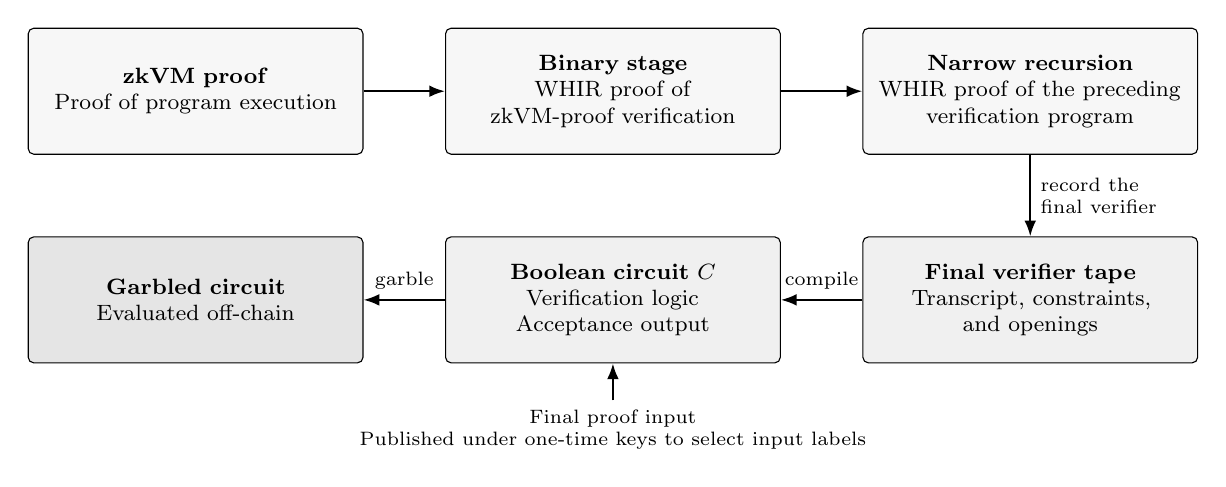
\begin{tikzpicture}[font=\footnotesize,
  box/.style={draw, rounded corners=2pt, text width=3.9cm,
    minimum height=1.6cm, align=center, inner sep=5pt},
  flow/.style={-{Latex[length=2mm]}, thick}]
\node[box, fill=gray!6] (shrink) at (0,0)
  {\textbf{zkVM proof}\\Proof of program execution};
\node[box, fill=gray!6] (binary) at (5.3,0)
  {\textbf{Binary stage}\\WHIR proof of\\zkVM-proof verification};
\node[box, fill=gray!6] (narrow) at (10.6,0)
  {\textbf{Narrow recursion}\\WHIR proof of the preceding\\verification program};
\node[box, fill=gray!12] (tape) at (10.6,-2.65)
  {\textbf{Final verifier tape}\\Transcript, constraints,\\and openings};
\node[box, fill=gray!12] (circuit) at (5.3,-2.65)
  {\textbf{Boolean circuit $C$}\\Verification logic\\Acceptance output};
\node[box, fill=gray!20] (gc) at (0,-2.65)
  {\textbf{Garbled circuit}\\Evaluated off-chain};
\draw[flow] (shrink) -- (binary);
\draw[flow] (binary) -- (narrow);
\draw[flow] (narrow) -- node[right, font=\scriptsize, align=left]
  {record the\\final verifier} (tape);
\draw[flow] (tape) -- node[above, font=\scriptsize] {compile} (circuit);
\draw[flow] (circuit) -- node[above, font=\scriptsize] {garble} (gc);
\node[font=\scriptsize, align=center] (input) at (5.3,-4.3)
  {Final proof input\\Published under one-time keys to select input labels};
\draw[flow] (input) -- (circuit);
\end{tikzpicture}
\caption{WHIR proofs of successive verification programs, followed by
compilation and garbling of the final verifier. In the Ziren implementation,
the initial zkVM proof is a shrink proof.
Arrows in the top row denote proof generation; those in the lower row denote
program transformations.
Binding a program and its outputs requires carrying their public-value digest
through the proof chain and binding it in the final statement; the measured
runs bind no public values.}
\label{fig:ziren-pipeline}
\end{figure}

\paragraph{Challenges.} Two problems stand between this idea and a
dispute that Bitcoin can settle.
\begin{itemize}
  \item[C1] \emph{Garbling the verifier.} Compiling the complete verification
    program must preserve its transcript, multi-table constraints and
    commitment checks in a circuit of fixed shape. The recorded verifier's
    assertions and operand types must remain enforced on circuit inputs, and
    the Fiat--Shamir schedule must match the reference implementation.
    Merkle authentication and transcript hashing also account for substantial
    circuit cost.
  \item[C2] \emph{On-chain data.} A STARK proof is about a thousand times a
    Groth16 proof, and in a dispute every bit of it is published under a
    one-time key: the selection material that reveals the bit, the script that
    authenticates it and the signature that binds it to the transaction.
    At a million input bits, publication requires millions of virtual bytes,
    compared with thousands of virtual bytes for Groth16-based designs.
\end{itemize}

\paragraph{Contributions.} We address both on-chain input cost (C2) and
off-chain garbling and verification cost (C1). The binary-field
verifier and garbling use hash-based assumptions; the underlying Ziren proof
and the transaction layer have the separate assumptions stated above.
\begin{itemize}
  \item \textbf{Bitcoin integration and on-chain cost (C2).} We place the
    verifier in a BitVM3-style dispute, state the label-selection task that
    publishing its input must solve, and price four one-time input schemes
    using signed transaction serializations for the final verifier input.
    We account for selection material, authentication
    script and transaction signature per bit and separate the measured
    one-key-set component from the unimplemented multi-copy soldering and
    transaction graph (\S\ref{sec:dispute}, \S\ref{sec:input}). The component
    measures 1.21\,MvB with the 8-bit adaptor baseline and 4.26--9.36\,MvB
    per hash-based key set for the final Ziren verifier's 564{,}552-bit input,
    against a few thousand virtual bytes for Groth16. We also
    serialize a hash-based construction that would match the adaptor cost
    under a batch opcode.
  \item \textbf{Circuit Input reduction (C2).} Narrow recursion over Ziren's binary
    stage reduces the final verifier's input to $564{,}552$ bits on real
    proofs, with cumulative configurations measured. The construction combines
    aligned narrow layouts, fixed-data specialization, compressed linear-form
    openings, shared reductions and commitment-parameter tuning
    (\S\ref{sec:reduce}, \S\ref{sec:eval}, Appendix~\ref{app:recursion}).
  \item \textbf{Circuit compilation of the recursive verifier (C1).}
    We translate the verifier produced by Ziren's binary stage and narrow
    recursion from a recorded program over $\F$ into a Boolean circuit with
    one acceptance output. The translation implements its arithmetic and
    hashing operations, preserves its equality and nonzero assertions, and
    constrains byte and selector operands. The recorded program includes the
    transcript, multi-table constraint verification and Boolean WHIR
    openings; correctness relies on Ziren's recorder
    (\S\ref{sec:tape}, \S\ref{sec:eval}).
  \item \textbf{Boolean arithmetic gadgets and Blake3 optimization (C1).}
    We implement Plonky3's existing Wiedemann tower arithmetic as Boolean
    circuits for free-XOR garbling, using recursive Karatsuba multiplication:
    $3^k$ \AND{} gates per $2^k$-bit product, with squaring and multiplication
    by the tower generator implemented using only \XOR{}s. We also optimize
    bitvm-gc's Blake3 circuit~\cite{bitvmgc} from $20{,}657$ to $10{,}281$ \AND{} gates per
    compression and add tree mode for long inputs
    (\S\ref{sec:gadgets}).
\end{itemize}
For the post-quantum goal, \S\ref{sec:pq} analyzes the STARK and garbling components in
the quantum random-oracle model, including Grover search on the garbling
offset, and distinguishes those bounds from the lower cut-and-choose level,
the underlying Ziren assumptions and the non-post-quantum transaction layer.
Section~\ref{sec:eval} estimates the complete WHIR-proof verifier's
garbling and input-publication costs across cumulative optimizations, and compares the
results with BitVM3's Groth16-based verification and the post-quantum
Bitcoin-bridge cost analysis of Tiwari and Feickert~\cite{tf26pq}.
The circuit translator and benchmark commands are open source;
Appendix~\ref{app:artifact} documents the availability limits of the
historical recursion implementation. The Blake3 circuit and a label-level evaluator are contributed to
GOAT's bitvm-gc~\cite{bitvmgc}.

% =====================================================================
\section{Related work}\label{sec:related}

We group prior work by how it verifies a proof on Bitcoin: by garbling a verifier,
by witness encryption, or through small pairing-based SNARKs that both approaches
rely on. We also discuss locally refutable verification and the garbling techniques we use.

\paragraph{BitVM.} BitVMX~\cite{bitvmx24} located a disputed
step of a general CPU's trace (RISC-V or MIPS) by an n-ary search over a hash
chain of the trace. ColliderVM~\cite{collidervm25} left the optimistic model: it
placed the computation on-chain in validity form and passed state between
transactions through hash-collision puzzles, without fraud proofs, at a script
length its authors estimate as nearly practical for STARK verification.
Delbrag~\cite{delbrag25} proposed replacing BitVM's fraud proof by the
off-chain evaluation of a garbled circuit whose outcome is revealed as a
secret, proving the circuit's correctness in zero knowledge. BitVM3 took up that idea and
garbled the verifier~\cite{bitvm3paper,che25sok}, defining BitVM3-CORE as a
sound and complete on-chain proof system with on-chain costs of about \$9.

\paragraph{Garbled verifiers.} The Boolean-garbled Groth16 verifier~\cite{bit25b}
has about $3\times10^9$ non-free gates and a 42\,GiB
garbled artifact~\cite{babe2026}. Garbling Groth16 with native
elliptic-curve group operations reduced the garbled program to
2.4\,MiB~\cite{kflt26native}. Glock~\cite{eag25glock} formalized garbled locks and
garbled a designated-verifier variant of Pari; BABE reported its garbled circuit at
about 12\,MB on a binary elliptic curve~\cite{babe2026}. GOAT's
bitvm-gc~\cite{bitvmgc} garbles Groth16 and a designated-verifier form of
Pari~\cite{garudapari} over BN254 and over the binary curve sect233k1.

We garble Ziren's final recursive verifier with bitvm-gc, and we contribute our
Blake3 circuit back to it. BitVM3's comparison of garbling schemes already listed a
Yao-style garbled STARK verifier, at about 10\,GB of off-chain storage and as an
estimate~\cite[Table~9]{bitvm3paper}; our compiled gate count gives
3.49\,GB per instance for the final WHIR-proof verifier from Ziren. TRAPGC-DV~\cite{trapgcdv26} verified Groth16 by designated evaluation:
the prover wraps its proof in an outer Groth16 proof under a per-session trapdoor
SRS and garbles a small circuit that checks it in scalar form, with
cut-and-choose and a universal-composability analysis. It too rests on pairings.

\paragraph{Garbling on Bitcoin} Futoransky, Larotonda and
Barbara~\cite{flb25} broke the authenticity of the RSA-based garbling proposed for
BitVM3 and of linear adaptors: coprime public exponents let the evaluator forge labels by
extended Euclid, and linear adaptors fall to the Franklin--Reiter related-message
attack. Our hash-based garbling has no such label algebra. Mosaic~\cite{mosaic26}
made cut-and-choose maliciously secure with an on-chain footprint independent of
the number of garbled copies, and Antichain Winternitz~\cite{antichain26} published
input labels on-chain at a cost up to $52.9\%$ lower than Lamport signatures. Both
are independent of the garbled circuit; \S\ref{sec:input} prices both for our
final verifier input.

\paragraph{Post-quantum Bitcoin bridges.} Tiwari and Feickert~\cite{tf26pq}
analyze the post-quantum cost of garbled-circuit Bitcoin bridges, including
the proof verifier and the on-chain encoding of its input labels. Their
estimates identify a tradeoff: hash-based STARK verification can reduce the
garbled artifact relative to a pairing-based verifier, while the larger
proof increases on-chain publication costs. We compare against a
representative STARK configuration from their analysis in
Table~\ref{tab:compare}. Our implementation addresses both costs by
compiling the complete WHIR-proof verifier from Ziren and reducing the
proof input consumed by that circuit.
QSB~\cite{levy26qsb}
constructed a hash-based, non-standard authorization path under existing
consensus rules, mined on mainnet in August 2026~\cite{starkware26qsb}; a
pre-signed, timelocked dispute graph is not yet within its reach.

\paragraph{Direct hash-based verification.} Bitcoin Wildlife Sanctuary's
Circle-STARK verifier~\cite{bitcoinwildlifecircle} implements field
arithmetic, FRI, Merkle paths and the Fiat--Shamir transcript in Bitcoin
Script, using \texttt{OP\_CAT} with \texttt{OP\_SHA256} for hashing.
StarkWare reports a Fibonacci-related proof verified on an
\texttt{OP\_CAT}-enabled Signet~\cite{starkware24computation}. This provides
an implemented alternative for hash-based proof verification. Its on-chain
Script execution and opcode requirement differ from our off-chain garbling
and input-publication approach. The reported demonstration does not provide
costs for the same final Ziren verifier, so we compare the architectures
without assigning it a numerical cost advantage. The STARK verification
uses hash-based assumptions; the covenant and transaction-authorization
mechanisms must be assessed separately for post-quantum security.

\paragraph{Locally refutable verification.} FlatChecks~\cite{lerner26flatchecks}
publishes a proof first and supplies the verifier's intermediate trace on
challenge; the dispute checks a named local condition. This offers a different
way to distribute verification across Bitcoin transactions. Our measured
publication mechanism authenticates every input label needed to evaluate a
complete garbled verifier. Comparing costs requires the same proof statement,
challenge path and publication boundary; we do not infer a numerical advantage
from the different applications reported in the two works.

\paragraph{Witness encryption.} BABE~\cite{babe2026} replaced the garbled
Groth16 verifier with witness encryption for linear pairing
relations~\cite{gkpw24}, making the one quadratic pairing linear with a small
garbled circuit built from decomposable randomized encodings on Argo
MAC~\cite{el26argo}: a 22\,MiB artifact per instance, on-chain cost
comparable to BitVM3~\cite{babe2026}. Deferred
binding~\cite{goatpbwe} extended it to public inputs known only at dispute
time with two further garbled circuits, at 0.92\,GiB per finalized instance,
768 input labels, an Assert of 2{,}154 bytes and a 14{,}312-byte
ChallengeAssert witness. Bitcoin PIPEs
v2~\cite{pipesv2} witness-encrypted a Schnorr signing key under an NP
statement to emulate covenants without a soft fork, with arithmetic affine
determinant programs~\cite{aadp2026,bij20adp} whose ciphertexts are cubic in
the constraint count, about 338\,TB for a 14{,}371-constraint pairing-SNARK
verifier, under a heuristic security analysis. All witness-encryption designs
are smaller off-chain than a garbled verifier, but all need a pairing SNARK,
so a STARK would first be wrapped in one, and none is post-quantum.

\paragraph{Binary-field proof systems and garbling.} Binius~\cite{dp25binius}
built succinct arguments over binary towers, and ring
switching~\cite{dp24ringswitch} turned a claim about a polynomial's bits into
one about its packed form; Plonky3's Boolean WHIR commitment~\cite{plonky3}, which we garble,
uses both with WHIR~\cite{whir25} as the proximity test, and its cheap
additions are what make a garbled verifier small. We use privacy-free
garbling~\cite{fno15privacyfree} with free-XOR~\cite{ks08}, one ciphertext per
\AND{} gate~\cite[\S6]{zre15} and the syntax of Bellare, Hoang and
Rogaway~\cite{bhr12foundations}; free-XOR rests on circular correlation
robustness~\cite{ckkz12freexor}. Witness encryption in general goes back to
Garg, Gentry, Sahai and Waters~\cite{ggsw13}.

\subsection{BitVM3-style verification}\label{sec:bitvm3}

 In BitVM3~\cite{bitvm3paper}, the
operator acts as the garbler and a challenger as the evaluator. At setup,
the operator garbles a proof-verification circuit. At dispute time, the
operator publishes the proof under one-time keys that reveal the selected
input labels. Any party holding the garbled circuit and these labels can
evaluate the verifier off-chain. An invalid proof yields a reject-output
label that unlocks an on-chain hashlock and prevents reimbursement. The
proof is public, so the garbling needs authenticity rather than privacy:
the evaluator may know the wire values but must not derive the label for
an incorrect output. Cut-and-choose checks the garbler's construction;
BABE~\cite{babe2026}, Mosaic~\cite{mosaic26} and bitvm-gc~\cite{bitvmgc}
use this approach. Our construction follows this division between off-chain
verification and on-chain input publication and refutation.

\subsubsection{Dispute graphs}\label{sec:disputegraph}

We describe transaction dependencies and execution conditions using the
UTXO transaction model~\cite[\S2.2 and Appendix~B.2]{laa25bitvm2}.

\begin{definition}[Dispute graph]\label{def:disputegraph}
A dispute graph is $\mathcal G=(V,E,\perp)$, where $V$ is a finite set of
transaction skeletons. A skeleton $T=(I_T,O_T)$ specifies the set $I_T$ of
input outpoints and the indexed collection $O_T$ of outputs, each with a
value and locking predicate. An edge
$(T,i,T')\in E$ means that $T'$ consumes output $i$ of $T$;
these dependencies are acyclic.
For distinct transactions, $T\perp T'$ means $I_T\cap I_{T'}\ne\varnothing$.
Let $U_0$ be the initial set of unspent outpoints. An execution of $n$
transactions is a sequence
$(T_k,\omega_k,h_k)_{k=0}^{n-1}$, where $T_k\in V$, $\omega_k$ is its
witness and $h_k$ its confirmation height. Let $U_k$ denote the set of
unspent outpoints after the first $k$ transactions. The execution is valid
if, for every $0\le k<n$,
\[
  \begin{gathered}
  U_k\xrightarrow{T_k,\omega_k,h_k}U_{k+1}
  =(U_k\setminus I_{T_k})\cup\operatorname{Out}(T_k),\\
  I_{T_k}\subseteq U_k,\qquad
  \mathsf{Valid}(T_k,\omega_k,h_k;H_k)=1.
  \end{gathered}
\]
Here $H_k$ is the confirmed history before step $k$, $\operatorname{Out}(T)$
is the set of newly created outpoints, and
$\mathsf{Valid}$ includes value conservation with fees, witness checks,
authorization and absolute or relative timelocks. Initial funding outputs
may be created by transactions outside $V$.
\end{definition}

This definition distinguishes a dependency graph from an execution: a
transaction with several parents requires all its inputs, and independent
publication branches may execute in either order. Conflicting transactions
cannot both occur in one valid history. A timeout is a lower bound on the
height at which a competing spend becomes valid; it does not itself cancel
another branch. Cancellation requires consuming an input needed by that
branch. Covenant emulation must additionally prevent unauthorized spends
of the protected outputs; graph notation alone does not enforce that
property.

\paragraph{Refutation predicate.} The refutation witness is a reject-output
label from a kept garbled verifier. Let $\ell^j_0$ denote the reject-output
label of kept instance $j$, and let $h_j=\mathrm{SHA256}(\ell^j_0)$ be its
committed hash. For a candidate label $\ell$, the refutation condition is
\[
  \mathsf{Reject}_j(\ell)
  :=\mathbf{1}\{\mathrm{SHA256}(\ell)=h_j\}.
\]
Here $\mathbf{1}\{\cdot\}$ is 1 when its condition holds and 0 otherwise.
Circuit authenticity and cut-and-choose relate this hashlock witness to an
invalid verifier input (\S\ref{sec:security}); the transaction graph
controls how its disclosure prevents reimbursement.

\paragraph{Dispute transitions.} Figure~\ref{fig:graph} shows the dispute
graph. Let $h_K$, $h_C$ and $h_A$ denote
the confirmation heights of Kickoff, Challenge and completed input
publication. Let $\Delta_C$, $\Delta_A$ and $\Delta_D$ be the challenge,
input-publication and refutation delays, respectively, measured in blocks
from these three heights. For an encoded verifier input $x$ partitioned
into $k$ chunks $x^{(1)},\ldots,x^{(k)}$ of fixed layout, define
\[
  \mathsf{Complete}(x)
  :=\bigwedge_{i=1}^{k}\mathsf{Auth}_i(x^{(i)}),
\]
where $\mathsf{Auth}_i$ requires publication and authentication of the
prescribed chunk and its binding to the same dispute instance. The chunks
must cover every input wire. Table~\ref{tab:graph-transitions} specifies the
required transition guards. The conditions on unspent connectors encode
conflicts, rather than asking Script to prove the absence of a transaction.

\begin{table}[t]\centering\small
\begin{tabularx}{\textwidth}{lX}\toprule
transition & required guard and effect\\\midrule
Kickoff $\to$ Take1 & $h\ge h_K+\Delta_C$ and the challenge connector remains
unspent; reimburse the operator.\\
Kickoff $\to$ Challenge & Spend the challenge connector and supply the
challenge bond; disable Take1.\\
Challenge $\to$ completed Assert & Publish all authenticated chunks so that
$\mathsf{Complete}(x)=1$, and create the completion output while its
required inputs remain unspent.\\
Challenge $\to$ AssertTimeout & $h\ge h_C+\Delta_A$ and a connector needed
for completion remains unspent; penalize the operator and disable completion.\\
completed Assert $\to$ Disprove$_j$ & Supply $\ell$ with
$\mathsf{Reject}_j(\ell)=1$ and consume a connector required by Take2;
prevent reimbursement.\\
completed Assert $\to$ Take2 & $h\ge h_A+\Delta_D$ and every required
refutation connector remains unspent; reimburse the operator.\\\bottomrule
\end{tabularx}
\caption{Transition guards and effects for the garbled-verifier dispute. The
publication subgraph must enforce completion before either terminal branch.}
\label{tab:graph-transitions}
\end{table}

The challenge and refutation windows provide time for a competing spend to
confirm; after a timelock matures, unresolved branches may race for the
same input. Safety and progress therefore also require ledger-confirmation
and honest-monitoring assumptions. The publication fanout or chain, its
completion and timeout connectors, and fee-management transactions remain
to be instantiated. Our fixtures in \S\ref{sec:eval} measure publication
components; they do not establish that the complete graph realizes these
transition guards.

\begin{figure}[t!]\centering
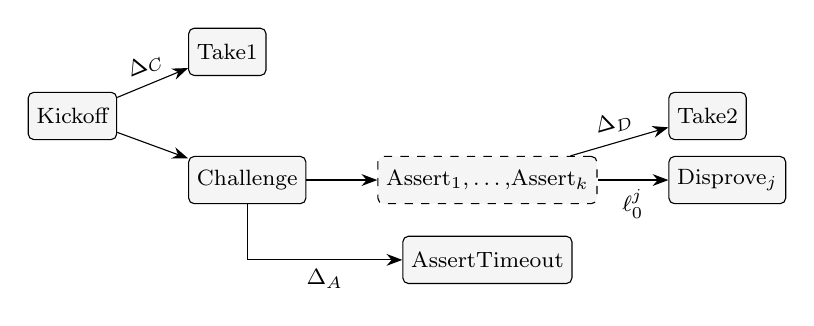
\begin{tikzpicture}[node distance=5mm and 9mm, font=\footnotesize,
  tx/.style={draw, rounded corners=2pt, minimum height=6mm, inner sep=3pt, fill=gray!8},
  arr/.style={-{Stealth[length=2mm]}}]
\node[tx] (kick) {Kickoff};
\node[tx, above right=2mm and 9mm of kick] (take1) {Take1};
\node[tx, below right=2mm and 9mm of kick] (chal) {Challenge};
\node[tx, dashed, right=of chal] (assert) {Assert$_1,\dots,$Assert$_k$};
\node[tx, above right=2mm and 9mm of assert] (take2) {Take2};
\node[tx, right=of assert] (disprove) {Disprove$_j$};
\node[tx, below=4mm of assert] (noassert) {AssertTimeout};
\draw[arr] (kick) -- node[above, sloped] {$\Delta_C$} (take1);
\draw[arr] (kick) -- (chal);
\draw[arr] (chal) -- (assert);
\draw[arr] (chal) |- node[pos=0.75, below] {$\Delta_A$} (noassert);
\draw[arr] (assert) -- node[above, sloped] {$\Delta_D$} (take2);
\draw[arr] (assert) -- node[below] {$\ell^j_0$} (disprove);
\end{tikzpicture}
\caption{Dispute graph. The dashed Assert$_1,\ldots,$Assert$_k$ node
groups the input-publication transactions.}
\label{fig:graph}
\end{figure}

\subsubsection{Setup and dispute}\label{sec:dispute}

\paragraph{Measurement scope.} We use \emph{total on-chain footprint}
to mean the sum of the virtual transaction sizes, in virtual bytes (vB), of
every transaction in the dispute graph, including ordinary transaction
signatures, authentication signatures or preimages, witness framing, revealed
tapscripts, control blocks, transaction inputs and outputs, anchors, timeouts
and fee-management transactions. A transaction's virtual size is its weight
divided by four, rounded up to an integer~\cite{bip141}; it differs from
the transaction's serialized size in bytes. We measure the input-publication component
of that footprint: bounded funding--reveal publication slices for all four
schemes, and a signed join for Lamport. The challenge, timeout, Disprove,
anchor and fee-management branches, the hash-based soldering across the kept
garblings and the binding of public values are not constructed, so the
figures are components of that footprint and conditional projections.

\paragraph{Setup.} Let $C$ be the proof-verification circuit with one
acceptance output, $N$ the total number of garbled instances and $M$
the number retained for evaluation, with $1\le M<N$.
The operator garbles $N$ instances of $C$ from independent
seeds and commits, for every instance $j$, the hash of its garbled tables,
$h_j=\mathrm{SHA256}(\ell^j_0)$ for the label of output value 0 (reject), and
the hashes of its one-time keys and label translations. A challenger chooses
$N-M$ instances to open, re-garbles each from its seed and checks every
commitment;
only then is the transaction graph signed, by a committee as in
BitVM2~\cite{laa25bitvm2}, whose enforcement requires at least one honest
signer to delete its signing key after setup.

Publishing bit $b$ of input $i$ must give a challenger only the label of value
$b$ on wire $i$ in every kept instance; Mosaic provides this correlation for
its adaptor-signature path~\cite{mosaic26}, and the hash-based soldering is
open here.

Section~\ref{sec:disputegraph} formalizes the dispute graph and its
transition guards. Its Assert node represents the input-publication subgraph.

\paragraph{Intended dispute.} The operator's Kickoff claims a reimbursement;
a challenger may spend its challenge output within $\Delta_C$, after which the
operator must publish every authenticated input bit through Assert or lose
its stake on timeout. A challenger then reads the published bits, derives
the input labels of every kept instance and evaluates each off-chain, one
Blake3 call per non-free gate. An
invalid proof yields $\ell^j_0$ from a correctly garbled instance, which opens
Disprove$_j$. The circuit size affects off-chain evaluation, while the proof
size controls the Assert payload. The historical Ziren recursion
measurements bind no external public values, so binding the withdrawal and
rollup-state commitment into the AIR relation and transcript, which a bridge
needs, is unimplemented and outside the reported figures. What Assert
publishes is the verifier's input, so the quantities to reduce are its bit
count, which the circuit fixes, and the script and signature bytes that each
bit costs, which the publication scheme fixes. Section~\ref{sec:protocol} develops these cost reductions.

% =====================================================================
\section{Setting}\label{sec:setting}

\subsection{Garbled verifiers on Bitcoin}

Let $C$ be the agreed proof-verification circuit with one output wire.
The operator garbles $C$, and a challenger evaluates it on the labels of the
published input $x$. We use \emph{privacy-free} garbling: the evaluator may
learn every wire's value. The required property is \emph{authenticity}:
given the labels of $x$, the evaluator obtains the label for $C(x)$ but
cannot derive the label for $1-C(x)$. The reject-output label is the witness
for the hashlock defined in \S\ref{sec:disputegraph}.

\subsection{The garbling scheme}\label{sec:garbling}

We use privacy-free garbling~\cite{fno15privacyfree} with free-XOR~\cite{ks08}
and one ciphertext per non-free gate, in the syntax of Bellare, Hoang and
Rogaway~\cite{bhr12foundations}.

Let $\Delta$ be a random
secret 128-bit offset. Every wire $w$ has a false label $w_0$, and its true label
is $w_1=w_0\oplus\Delta$. Let $H(\ell,g)=\blake(\ell\,\|\,g)$ truncated to 128
bits, where $g$ is the gate's index. An \XOR{} gate sets $c_0=a_0\oplus b_0$ and
has no ciphertext. An \AND{} gate $c=a\wedge b$ sets
\[
  c_0 = H(a_0,g), \qquad \mathit{ct} = H(a_1,g)\oplus H(a_0,g)\oplus b_0 .
\]
The evaluator recovers the output label from its two input labels, the
ciphertext and one hash~\cite[\S6]{zre15}; an \textsf{OR} gate is symmetric. The
garbled circuit is one 16-byte ciphertext per non-free gate.

Two details matter in practice. First, $\Delta$ must be secret and fresh for
each garbling: with a public $\Delta$ any label yields its complement, and the
output's other label is free to compute. Second, a hash modeled as circular correlation
robust (\S\ref{sec:security}) gives labels no algebraic structure. RSA-based garbling proposals for BitVM3 were broken
exactly through such structure: label forgery by extended Euclid on coprime
exponents, and by the Franklin--Reiter related-message
attack~\cite{flb25}.

\subsection{The target verification program}

Our target computation is the complete verifier of a WHIR-based STARK proof
from Ziren, abbreviated as a \emph{WHIR proof}. This includes the AIR and cross-table
checks as well as the WHIR opening proof that authenticates polynomial
evaluations. In our Ziren implementation~\cite{duan26ziren}, the binary
stage proves execution of the shrink-proof verifier over $\F$ using Boolean
WHIR and Blake3. Subsequent narrow recursion reduces the cost of the final
WHIR-proof verifier that we compile into a Boolean circuit and garble
(\S\ref{sec:eval}). This binary-field
verification backend is implemented in Plonky3~\cite{plonky3} and uses fields in the
Wiedemann tower~\cite{wiedemann88}
\[
  \T_0=\mathbb{F}_2,\qquad \T_{k+1}=\T_k[X_k]/(X_k^2+X_{k-1}X_k+1),\qquad X_{-1}=1 ,
\]
up to $\T_7=\F$. An element of $\T_{k+1}$ is stored as its low half (the
coefficient of $1$) and its high half (the coefficient of $X_k$), recursively
down to bits. The trace is committed as bits: a Boolean column is packed into
$\F$ elements, and WHIR uses Reed--Solomon proximity testing to authenticate the packed
multilinear polynomial on an additive (Cantor) evaluation
domain~\cite{whir25,cantor89,lch14}. Binary towers and
ring switching come from Binius~\cite{dp25binius,dp24ringswitch}.

\paragraph{Verification predicate.} The Boolean circuit $C$ implements the
acceptance predicate of the final WHIR proof, including its
transcript and all verification constraints, and produces a single acceptance
bit. We garble $C$ for evaluation in the dispute protocol
(\S\ref{sec:garbling}).

The verification program for this WHIR proof comprises the following
stages:
\begin{enumerate}
  \item \emph{Transcript reconstruction.} Absorb the preprocessed and main
    trace commitments and the declared public values, and derive Fiat--Shamir
    challenges in the prescribed order throughout verification. The algebraic
    intermediate representations (AIRs) specify polynomial constraints on
    current and next trace rows; these constraints, the table dimensions
    and the verifying key determine the expected proof structure.
  \item \emph{Cross-table consistency.} Verify the binary-bus product
    argument linking the recursion machine's tables, together with any lookup
    reductions required by the configured AIRs. The resulting evaluation
    claims must subsequently be bound to committed trace values.
  \item \emph{Constraint reduction.} Verify the shared \emph{zerocheck}
    sumcheck~\cite{hyperplonk23,lfkn92}, which reduces the claim that AIR
    and bus constraints vanish on every row to a check at a common random
    evaluation point. Each table uses the coordinates corresponding to its trace height;
    any indexed lookup reduction is verified at its prescribed points.
  \item \emph{Opening reduction.} Reduce the required evaluations of main
    and preprocessed columns, or their linear forms, to claims on the packed
    trace polynomials. This includes the column-batching sumchecks and the
    bit ring-switch arguments over $\F$.
  \item \emph{Commitment verification.} Verify the Boolean WHIR openings
    for those claims, including the sumcheck rounds, grinding checks, STIR
    queries~\cite{stir24} that open folded codewords at random positions,
    Merkle authentication paths and final-polynomial checks. Main
    values are bound to the proof's trace commitment, and preprocessed values
    to the commitment fixed by the verifying key.
  \item \emph{Constraint closure.} Evaluate the AIR and bus constraints
    using the authenticated openings, discharge the remaining lookup claims,
    and check consistency with the sumcheck's terminal claim. The circuit
    returns acceptance only if these checks and all assertions introduced by
    the Boolean translation hold.
\end{enumerate}
All challenges come from a Blake3~\cite{blake3spec} sponge over bytes, and all
Merkle trees use Blake3 compressions.

% =====================================================================
\section{Construction and optimizations}\label{sec:protocol}

Two quantities determine the principal costs of our garbled WHIR-proof
verifier: the number of published input bits and the number of non-free gates. The former
controls input authentication on Bitcoin; the latter controls garbling,
evaluation and garbled-table storage. Within the BitVM3 framework of
\S\ref{sec:bitvm3}, we develop Boolean compilation and gate reductions
(\S\ref{sec:construction}), input publication (\S\ref{sec:input}), and
recursion and proof reductions (\S\ref{sec:reduce}). These optimizations
trade prover work, circuit size and input length; we state those tradeoffs
explicitly. Appendix~\ref{app:protocol} details the input-authentication schemes,
and Appendix~\ref{app:recursion} gives the algebraic arguments.

\subsection{Boolean compilation and off-chain verification cost}\label{sec:construction}

The circuit sets the first quantity: it reads the proof's bits, so its input
layout is the bit count that Assert publishes. Its size is also what
cut-and-choose garbles and challengers store. This subsection turns the
verifier of \S\ref{sec:setting} into a Boolean circuit with one output wire.
We first describe how the recursive verifier is recorded and compiled, then
the arithmetic and hash gadgets that reduce its non-free gate count.

\subsubsection{Verifier recording and circuit compilation}\label{sec:tape}

Ziren's binary stage proves the execution of the program that verifies a
Blake3-committed shrink proof. Its verifier is recorded as a straight-line
tape of operations over $\F$. A five-table machine, comprising ledger,
arithmetic, rewiring, hash and Blake3-round tables, proves an execution of
that tape. Recording and proving the resulting verifier repeats this narrow
recursion; the circuit we garble is compiled from the final verifier tape.
The recorder captures the multi-STARK verification program, including its
transcript, AIR and bus constraints, preprocessed data and commitment
openings. Recording and proof-system optimizations are developed in
\S\ref{sec:reduce}.

Our \texttt{binary\_tape} translator implements each tape instruction with
Boolean gates. Field addition and squaring use \XOR{}s; multiplication uses
the tower gadget, and inversion uses an addition chain with a nonzero check.
Equality and nonzero assertions become check bits. Byte conversions and
selectors enforce their operand ranges, while hash instructions use the
Blake3 circuit and Merkle instructions select the order of the two child
digests before hashing. Inputs are encoded according to their use as bits,
bytes or 128-bit field elements. All assertion and range-check bits are
conjoined into one acceptance output. The circuit shape is fixed by the
recorded tape and its input types; the translation relies on the recorder to
capture the reference verifier faithfully.

\paragraph{Streaming execution.} We use bitvm-gc's streaming backend~\cite{bitvmgc} for
the compiled verifier. A planning pass determines wire lifetimes;
the streaming pass reuses storage after a wire's final use, retaining the
acceptance output. This reduces the live-label memory required to execute
the circuit without changing its gates or input. Planning metadata and the
stored garbled tables remain separate costs. In particular, streaming does
not remove the challenger's obligation to retain the kept garblings.

\paragraph{Why a binary field.} The binary stage and narrow recursion use
Boolean WHIR commitments over $\F$, whose addition is \XOR{} and hence free
under free-XOR. A field multiplication costs $2{,}187$ \AND{} gates by
Karatsuba down the tower, while squaring and multiplication by the tower
generator are free. The bit ring switch of Binius~\cite{dp24ringswitch}
reduces bit-level claims to claims on the packed $\F$ polynomial. The resulting opening reductions are further combined in
\S\ref{sec:reduce}.

\paragraph{Why Blake3.} One hash serves three roles: the Merkle commitments
and the Fiat--Shamir sponge of the proof system, and the garbling hash $H$ of
\S\ref{sec:garbling}. Blake3 is an add-rotate-XOR design, so in Boolean gates
its only non-free operations are the 32-bit additions, one \AND{} per bit with
the carry gadget of \S\ref{sec:gadgets}. For comparison, our Boolean implementation of a width-16 Poseidon2
permutation over KoalaBear~\cite{poseidon2} uses 1{,}240{,}747 \AND{} gates,
about 120 Blake3 compressions. A prover that already commits and samples with Blake3 needs
no change, and the circuit's transcript can be checked byte for byte against
it. A single hash also keeps the
verifier's assumptions to those of \S\ref{sec:security}, Blake3 as a random
oracle with circular correlation robustness, with no elliptic-curve or lattice
assumption, which is what makes the verifier's own security claim
post-quantum (\S\ref{sec:pq}).

\subsubsection{Gadgets}\label{sec:gadgets}

\paragraph{Tower arithmetic.} We retain Plonky3's Wiedemann tower
representation~\cite{plonky3,wiedemann88} and translate its reference
arithmetic into Boolean gates. A wire vector for an element of $\T_k$ is its
bit pattern, so gadget outputs can be read back directly as field elements.
Multiplication follows the existing tower algorithm recursively, using
Karatsuba at each level. For
$a=a_0+a_1X_k$ and $b=b_0+b_1X_k$ in $\T_{k+1}$, with
$a_0,a_1,b_0,b_1\in\T_k$, define the intermediate products
\[
  z_0=a_0b_0,\quad z_2=a_1b_1,\quad z_1=(a_0+a_1)(b_0+b_1)+z_0+z_2,\qquad
  ab=(z_0+z_2)+(z_1+X_{k-1}z_2)\,X_k .
\]
Additions are free. Multiplication by the generator $X_{k-1}$ is a rewiring plus
\XOR{}s, and squaring is linear over $\mathbb{F}_2$. The only \AND{} gates are
the base-field products, three per level, so a $2^k$-bit multiplication costs
$3^k$ \AND{} gates: $2{,}187$ in $\F$. A multiplication by a constant folds to
\XOR{}s entirely.

\paragraph{Blake3.} We start from bitvm-gc's Blake3 circuit~\cite{bitvmgc} and change two
things. A 32-bit addition's carry is the majority
\[
  \mathrm{maj}(a,b,c)=c\oplus\big((a\oplus c)\wedge(b\oplus c)\big),
\]
where $a,b$ are the operand bits and $c$ is the incoming carry. This uses
one \AND{} per bit, and the carry out of the top bit is discarded, so it is not
computed. This halves a compression from $20{,}657$ to $10{,}281$ \AND{} gates.
We also add Blake3's tree mode (chunk chaining values on a stack, parent nodes,
the root last). Tree mode supports transcript messages that exceed one 1{,}024-byte
chunk between samples. Table~\ref{tab:gadgets} gives the costs. Every gadget is checked
against reference implementations of the field and the hash on random inputs.

\begin{table}[t]\centering\small
\begin{tabular}{lr}\toprule
gadget & \AND{} gates\\\midrule
$\F$ multiplication & 2{,}187\\
$\F$ squaring, tower-generator multiplication, addition & 0\\
Blake3 of 64 bytes (a Merkle compression) & 10{,}281\\
Blake3 of 256 bytes (a leaf row of 16 elements) & 41{,}511\\
Blake3 of 1{,}072 bytes (two chunks: a transcript flush) & 186{,}125\\\bottomrule
\end{tabular}
\caption{Gadget costs, checked against reference implementations of the field
and the hash.}
\label{tab:gadgets}
\end{table}

\subsection{Publishing the input}\label{sec:input}

\paragraph{Label selection.} Every input mechanism we price is an instance of
one two-party task. The \emph{garbler} $\mathsf{G}$ (the operator, who also
proves) holds the two labels $\ell_w^0,\ell_w^1$ of every input wire $w$ of the
kept garblings; the \emph{evaluator} $\mathsf{E}$ (a challenger) will run the
garbled verifier on the proof $\pi$. Write $\pi_w$ for bit $w$ of its fixed
circuit-input encoding; instance indices are suppressed in $\ell_w^b$.
Publishing $\pi$ on-chain must
(i)~\emph{deliver} $\ell_w^{\pi_w}$ to $\mathsf{E}$ for every $w$, (ii)~be
\emph{exclusive}: an evaluator given the published input labels cannot
compute any $\ell_w^{1-\pi_w}$ without the garbler's secrets, since one
complementary label breaks authenticity (\S\ref{sec:security}), (iii)~be
\emph{binding}: $\mathsf{G}$ publishes at most one value per wire, and the
publication is also the authorization of the spending transaction, and (iv)~be
\emph{public}: any observer can recover $\pi$ and check the published object.

A malformed publication cannot be spent, a missing one forfeits the stake
through AssertTimeout, and Disprove is reserved for the reject label. Lamport
signatures~\cite{lamport79} achieve (i)--(iv) with one preimage per bit, at the cost of a per-bit script.
The Schnorr adaptor baseline of BitVM3 and Mosaic~\cite{bitvm3paper,mosaic26}
achieves them with one signature per $k$-bit digit and no per-bit script;
Appendix~\ref{app:adaptor} gives its protocol diagram
(Figure~\ref{fig:adaptorseq}). The hash-based alternative
(Figure~\ref{fig:hashseq}, Appendix~\ref{app:hashsel}) replaces the signature
by a pair of hash-chain openings and underlies the Antichain row and the
hash-based projections of \S\ref{sec:pq}.

The adaptor uses one \texttt{CHECKSIG} per digit for both selection and
transaction binding. Hash-based schemes additionally authenticate their
openings with hash ladders and require a separate transaction signature.
For the final verifier's 564{,}552-bit input, these differences give
1.21\,MvB for the adaptor baseline and 4.26--9.36\,MvB for the hash-based
schemes (Table~\ref{tab:ziren-publication}). Table~\ref{tab:bytes} breaks
down their costs per digit or bit. Appendix~\ref{app:pqsel} separately
considers a hash-based batch-verification opcode.

\begin{table}[t]\centering\footnotesize\setlength{\tabcolsep}{4pt}
\begin{tabularx}{\textwidth}{>{\raggedright\arraybackslash}p{2.2cm}>{\raggedright\arraybackslash}p{3.7cm}>{\raggedright\arraybackslash}p{2.9cm}>{\raggedright\arraybackslash}p{2.6cm}r>{\raggedright\arraybackslash}X}\toprule
scheme & selection material & script & transaction binding & vB/bit & assumption\\\midrule
Schnorr adaptor, $k=8$ & one 64-byte completion per 8-bit digit & one \texttt{CHECKSIG} per digit, 3 bytes & the same signature & 2.13 & discrete logarithm\\
WOTS translation, $k=3$ & one 20-byte chain node per 3-bit digit, plus two checksum chains per chunk & hash ladder in Script, 2 bytes per step & separate 64-byte Schnorr signature per input & 7.55 & hash; 128-bit translation chain\\
Antichain $(2,16)$, $k=4$ & two 20-byte chain nodes per 4-bit digit & hash ladder in Script, 2 bytes per step & separate 64-byte Schnorr signature per input & 11.38 & hash\\
Lamport & one 16-byte preimage per bit & 49 bytes per bit & separate 64-byte Schnorr signature per input & 16.59 & hash\\\bottomrule
\end{tabularx}
\caption{Where the four input schemes spend their bytes. Selection material
and script are per digit or per bit as stated; vB/bit is the measured
one-key-set component of Table~\ref{tab:ziren-publication}, including transaction
shells. The adaptor's selection and binding are one object, which is why its
script is three bytes per digit; the hash-based schemes pay for the ladder in
Script and for a separate signature, and only their selection is hash-based.}
\label{tab:bytes}
\end{table}

\paragraph{One-time signature schemes.} We price four one-time schemes for carrying
the input bits; Appendix~\ref{app:schemes} gives their scripts and fixtures and
Table~\ref{tab:ziren-publication} their sizes. \emph{Lamport} reveals one of two hashed
16-byte preimages per bit against a 49-byte leaf script, 998 bits per input,
with a 32-byte authorization key and \texttt{OP\_CHECKSIGVERIFY} prefixed to
each leaf. \emph{Antichain Winternitz}~\cite{antichain26} closes the
forward-hashing gap of plain Winternitz chains at a cited marginal 11.31\,vB
per bit at parameters $(2,16)$; our fixture pins the upstream implementation
and adds a 64-byte Schnorr authorization. \emph{Winternitz with a translation
table}~\cite{wotstranslation26} closes the same gap by making each label a
Shamir secret whose threshold a signed chunk's checksum sets; our fixture uses
3-bit digits, eight per chunk. For the final Ziren input, the off-chain
translation table occupies 1.03\,GB per instance
(Table~\ref{tab:compare}).

\emph{Schnorr adaptor signatures} over 8-bit digits, as in BitVM3
and Mosaic~\cite{bitvm3paper,mosaic26}, yield 9{,}323 weight units per
1{,}024-bit Assert shell in our fixture, which validates every completed
signature under Core 31.1; the signatures
rest on discrete logarithms, and this repository does not implement Mosaic's
polynomial soldering. Increasing the digit width reduces the number of
on-chain signatures but expands the off-chain choice table exponentially;
we retain the 8-bit construction as the authenticated baseline.

Our labels are free-XOR correlated, so a hash-based preimage $s$ cannot itself
be a label: a key-derivation function (KDF) maps it to one by a translation
ciphertext $\mathrm{KDF}(s)\oplus w_b$, two per input bit and instance,
18.07\,MB for the final verifier's 564{,}552-bit input. Using one on-chain key set for all $M$ kept
instances requires a proof that the translations of opened and kept instances
encode the same bit choices. BABE's zero-knowledge soldering~\cite{babe2026}
and Glock's verifiable secret sharing~\cite{eag25glock} give related mechanisms
at smaller input sizes; we have neither constructed nor costed one for
our input, so the one-key-set hash rows of Table~\ref{tab:ziren-publication} are
conditional on it. The soldering-failure probability
$\varepsilon_{\mathrm{sol}}$ has no instantiated bound.
Authenticating each input independently for every kept instance instead
multiplies the component by $M$: for the final Ziren input at $M=7$,
65.54\,MvB for Lamport, 44.98\,MvB for Antichain and 29.84\,MvB for WOTS
translation, before graph
overhead and still without enforcing the same bit choice across the sets.

\subsection{Reducing recursive-proof inputs and verification work}\label{sec:reduce}

The circuit consumes only the proof values read by the final verifier tape.
We reduce that input at three levels: the recursion machine's layout, the
representation of its opening claims, and commitment authentication. Some
changes also eliminate non-free gates; others add verification work to save
published bits. Table~\ref{tab:recursion} reports the cumulative measured
configurations, including changes evaluated together rather than in isolated
ablations. The following mechanisms apply to the Ziren recursion path.

The opening reductions connect the values used by AIR and bus checks to
the committed trace. A column sumcheck~\cite{lfkn92} reduces claims about
linear combinations of columns to column evaluations at random points.
The bit ring switch~\cite{dp24ringswitch} translates those claims into the
packed-field representation authenticated by WHIR~\cite{whir25}. The
optimizations below reduce the values and round messages carried between
these steps. Each transmitted field element adds 128 circuit-input bits;
processing it also incurs transcript and verification work. The final
commitment openings remain necessary to authenticate the reduced claims.

\subsubsection{Narrow recursion and aligned trace layouts}

\paragraph{Recursing over the verification program.} The binary stage proves
execution of the complete shrink-proof verifier. Each subsequent level
proves execution of the preceding verifier in the five-table machine of
\S\ref{sec:tape}. The final garbled circuit therefore verifies a proof of a
narrow machine rather than exposing the original verification program's
trace width at its input. This reduces final-verifier input and gate counts
by moving work into recursive proof generation. Our cost evaluation focuses
on garbling and evaluating the final verifier and publishing its inputs.

\paragraph{Aligned table packing.} A power-of-two table block placed at an
offset aligned to its own size needs one ring-switch claim. An unaligned
block can split into several claims, each carrying a tensor and its
verification work. We align the narrow machine's power-of-two blocks and
pad its preprocessed round-table width accordingly. This removes split
claims before the later claim-merging step. An aligned block has a fixed
address prefix and free trailing coordinates, so one restriction of the
packed polynomial describes the entire block. A block crossing such an
address boundary needs several restrictions, which explains the additional
claims. The layout change applies to the narrow machine; it does not impose this alignment on the binary stage's
arbitrary table layouts.

\paragraph{Narrow rewiring rows.} We reduce the rewiring table's row width
from 128 bytes to 64 bytes. A transpose gathers halves separately and uses
arithmetic additions to join disjoint halves; the bus authenticates those
halves. Fewer columns require fewer opened field values, but the extra
arithmetic rows increase prover work. Thus narrowing the machine is a
tradeoff between final verification cost and the size of the execution trace
that recursion must prove.

\subsubsection{Specializing fixed data and input encodings}

\paragraph{Typed inputs and known values.} The translator allocates one bit,
eight bits or 128 bits according to a consumed input's type, while enforcing
its byte and selector ranges. Unread proof values receive no input wires.
The recorder also replaces known padding values and preprocessed columns
constant over every row with circuit constants, after checking their values
in the recording proof. Their transcript absorption and commitment-opening
relations remain checked; the substitution removes input wires rather than
omitting the corresponding verification constraints. Constant field
multiplications then reduce to \XOR{}s.

\paragraph{A deep cap for fixed preprocessing.} The preprocessed Merkle tree
is fixed by the verifying key. We embed its nodes at a chosen depth as
constants, checked against the key's cap, and select the appropriate node
using a one-hot decoding of the query index. A query authenticates only the
path below that node, so upper siblings are no longer circuit inputs and
their hashes are no longer computed. The verifier still hashes the
query-dependent leaf and lower path to a selected constant node. Each
omitted upper sibling saves one digest from the input and one path hash;
the one-hot selector enforces which embedded node the query reaches.
Greater depth adds selection gates:
the historical final configuration uses depth 18, whose input saving comes
with a small increase in total gates (Table~\ref{tab:recursion}). This
specialization depends on the fixed preprocessing tree; proof-dependent
main commitments cannot be treated as constants.

\subsubsection{Opening only the linear forms used by verification}

\paragraph{Packed operands and general linear forms.} The ledger's values
and arithmetic operands are read by their constraints and buses as packed
field elements. We first replace each such group of column openings by its
packed value. We then generalize this compression: symbolic AIR and bus
expressions determine a fixed matrix $L$ of required linear forms. Instead
of transmitting the full column-evaluation vector $x$, the prover sends
the vector $y=Lx$ of linear-form evaluations. For example, if the affected
checks use two columns only through $x_0+\gamma x_1$, for a fixed
coefficient $\gamma\in\F$, one transmitted field element can replace the
two column evaluations. The extractor must retain every additional
combination read elsewhere by a constraint or bus.
The verifier reconstructs a representative $Ry$ using a fixed right inverse
$R$ on the image of $L$, so $LRy=y$ for $y\in\operatorname{im}L$.
This preserves an affected expression precisely when it factors
through $L$, as formalized in Lemma~\ref{lem:forms}. The reconstruction uses
constant field coefficients and therefore only \XOR{}s. A column sumcheck
binds the transmitted forms to the committed trace; fewer transmitted
values do not dispense with that authentication.

\paragraph{Affine relations in fixed preprocessing.} For preprocessed
columns, we additionally derive relations over every row of the fixed
trace, including the all-ones column in the basis. Dependent forms are
reconstructed from an independent subset and constants. Linearity of
multilinear extension preserves these affine identities at every opening
point. This removes further input values without guessing relations from
a particular proof's evaluations.

\paragraph{One shared forms sumcheck.} The forms must be checked against
the committed columns. Running a separate column sumcheck for each table
repeats the round messages and transcript updates. We instead batch the
form claims before running one sumcheck over the widest column domain.
Here a group $t$ contains the forms of one table block at a fixed row
point. Let $k_t$ be its column-variable count, $C_t$ the multilinear
column polynomial at that row point, and $L_{t,j}$ the multilinear
extension of the coefficient vector of form $j$. Its claimed value
$y_{t,j}$ must satisfy
\[
  y_{t,j}=\sum_{u\in\{0,1\}^{k_t}}L_{t,j}(u)C_t(u).
\]
The commitments, row points and claimed forms are absorbed before sampling
$\rho\in\F$. Enumerate all forms with distinct consecutive exponents
$e_{t,j}$ starting at zero, and define
\[
  Y=\sum_{t,j}\rho^{e_{t,j}}y_{t,j},\qquad
  W_t(u)=\sum_j\rho^{e_{t,j}}L_{t,j}(u).
\]
The combined claim is $Y=\sum_t\sum_u W_t(u)C_t(u)$. These random weights
prevent a fixed collection of false form claims from cancelling except
with the batching error accounted for in Lemma~\ref{lem:shared-forms}.

To share rounds across different widths, let
$d_{\mathrm{col}}=\max_t k_t$ and zero-extend both $W_t$ and $C_t$ to
$\{0,1\}^{d_{\mathrm{col}}}$. For $z\in\F^{d_{\mathrm{col}}}$, write $z_t$
for its trailing $k_t$ coordinates and define
$b_t(z)=\prod_{i=1}^{d_{\mathrm{col}}-k_t}(1-z_i)$. The shared integrand is
\[
  S(z)=\sum_t b_t(z)^2 W_t(z_t)C_t(z_t),\qquad
  Y=\sum_{u\in\{0,1\}^{d_{\mathrm{col}}}}S(u).
\]
The prefix is squared because both factors are zero-extended. On Boolean
points $b_t^2=b_t$, but the terminal point is a random field point, where
the square cannot be dropped. The integrand has degree at most two in
each variable, so every sumcheck round uses a quadratic polynomial.

Starting from running claim $s_0=Y$, round $i$ supplies a polynomial
$g_i(X)=A_i+B_iX+D_iX^2$ whose Boolean sum must equal $s_i$.
The prover sends only $A_i,D_i$; the verifier reconstructs
$B_i=s_i-2A_i-D_i$ to enforce $g_i(0)+g_i(1)=s_i$. After absorbing the
message, it samples $\alpha_i$ and sets $s_{i+1}=g_i(\alpha_i)$.
After $d_{\mathrm{col}}$ rounds, the challenges form $z$ and the verifier
checks $s_{d_{\mathrm{col}}}=S(z)$. It computes each $W_t(z_t)$ from the
known coefficients and batching weights, while the prover supplies the
column fold $C_t(z_t)$. Each fold becomes a ring-switch claim and is
subsequently authenticated against the commitment.

For $n_{\mathrm{grp}}$ groups, the reduction sends
$2d_{\mathrm{col}}+n_{\mathrm{grp}}$ field elements, excluding the forms
themselves, instead of $2\sum_t k_t+n_{\mathrm{grp}}$ for separate
sumchecks with the same round encoding. For example, 16-column and
8-column groups share four rounds instead of running four and three
rounds separately. The terminal fold for each group is retained. The
saving is in repeated messages and transcript work; the verifier still
computes the batched terminal relation. Lemma~\ref{lem:shared-forms} gives
the conditional algebraic bound, with commitment-authentication errors
accounted for separately.

\subsubsection{Combining ring-switch claims and shortening bus rounds}

\paragraph{Merged ring-switch tensors.} A ring-switch tensor connects a
claim on unpacked bits to their packed field representation. Several
claims can repeat this tensor message even when the coordinates absorbed
into each packed element are identical. In that case their tensors share
one linear reading map $\ell$. For tensors $T_0,\ldots,T_{m-1}$ with
claimed readings $y_i=\ell(T_i)$, bind the points and readings before
sampling $\mu\in\F$, and transmit
\[
  T=\sum_{i=0}^{m-1}\mu^iT_i,\qquad
  \ell(T)=\sum_{i=0}^{m-1}\mu^iy_i.
\]
Linearity makes the second equality the randomly weighted combination of
the original claims. The remaining tensor checks and sumcheck bind the
merged tensor to the packing. The implementation checks the shared-coordinate
condition and excludes successor views from this case, since a different
reading map would invalidate this combination. Sending one tensor saves
repeated tensor inputs and their verification work. The batching error
and the subsequent authentication are treated in Appendix~\ref{app:recursion}.

\paragraph{A joint main/preprocessed ring switch.} A trace has
proof-dependent main columns and fixed preprocessed columns. Opening them
through separate ring switches repeats the reduction transcript. We combine
equal-size main and preprocessed packings, whose multilinear extensions are $P_0$ and
$P_1$, respectively. For their common coordinate vector $z$ and a new
selector variable $s$, define
\[
  P(s,z)=(1-s)P_0(z)+sP_1(z).
\]
The selector $s$ identifies which half of the combined packing is read:
the original main and preprocessed claims enter at $s=0$ and $s=1$.
One ring switch over this enlarged domain reduces the combined claims
to a terminal point, where the paired WHIR opening authenticates
both $P_0$ and $P_1$ and the verifier checks their selector-weighted sum.
This removes a second ring-switch transcript while adding one selector
coordinate. Both commitments and both terminal openings are retained;
the saving comes from sharing their algebraic reduction. This operation
complements tensor merging: tensor merging combines compatible readings,
while the joint switch combines the main and preprocessed packing domains.

\paragraph{Eq-factored bus rounds.} The bus product argument reduces a
claim about products to claims about their children. In a radix-four layer,
the product of four multilinear child values has degree at most four in
the current sumcheck variable. Multiplication by the known equality weight
raises the round degree to five. We avoid transmitting the extra polynomial
data contributed by that known factor. The round polynomial has the form $g(X)=e_r(X)h(X)$, with known
linear factor $e_r(X)=(1-r)(1-X)+rX$ and $\deg h\le4$, where $r$ is the
current coordinate of the equality-polynomial challenge point. A
degree-five round normally needs five transmitted field elements after
using the Boolean-sum constraint. Factoring out $e_r$ leaves a degree-four
polynomial, which needs four transmitted elements once the same constraint
is used. From the running claim $s=g(0)+g(1)$, the verifier reconstructs the
omitted value as
\[
  h(1)=\frac{s-(1-r)h(0)}{r}.
\]
Since $e_r(0)=1-r$ and $e_r(1)=r$, this reconstruction enforces the
original Boolean-sum relation. The circuit requires $r\ne0$. After absorbing
the round message, it samples
the next sumcheck challenge $\alpha\in\F$ and advances the claim to
$e_r(\alpha)h(\alpha)$. Each round sends one fewer field element, at the
cost of reconstruction arithmetic, including the inverse of $r$. This
saves 128 circuit-input bits per affected round, but need not reduce the
non-free gate count. The verified polynomial still has
degree five; the shorter message does not lower its soundness error.
Appendix~\ref{app:recursion} gives the algebraic checks for these reductions.

\subsubsection{Commitment parameters and accelerated grinding}

\paragraph{Per-round WHIR scheduling.} WHIR~\cite{whir25} repeatedly
folds the committed polynomial, authenticates queried codeword values and
reduces verification to a smaller polynomial. Its proof input includes
opened leaf rows, Merkle siblings, out-of-domain (OOD) answers, sumcheck messages
and the final polynomial. OOD answers bind evaluations at points outside
the code's evaluation domain. Reducing one component can enlarge another, so
we select folding factors, code rates and grinding budgets jointly for the
recursive proof's shape.

A larger fold eliminates more variables in one stage and can remove later
stages, but can also widen the row opened by each query. A lower code rate
adds redundancy, which can reduce the query count required by the security
assessment, while enlarging the evaluation domain and its Merkle tree.
More grinding requires the prover to search for a transcript nonce, trading
hash trials for fewer queries under the chosen assessment. Every removed
query saves its leaf payload and authentication path; the garbled verifier
also avoids the corresponding path hashes. We score the complete opening
schedule, including round messages and terminal data, rather than minimizing
the number of queries alone. Since polynomial arity decreases through the
protocol, different folding factors can be preferable in different rounds.

The historical final configuration folds 4, 5, 4 and 4 variables with up to
46 bits of grinding. A schedule must fit the actual polynomial arity;
these historical parameters are not a
universal setting for other recursion traces.

\paragraph{Shorter Merkle digests.} We reduce each Blake3 Merkle digest
from 32 bytes to 25 bytes (256 bits to 200 bits). This directly
reduces proof input; it does not imply a proportional reduction in hash
gates. It also caps generic collision resistance at 100 classical bits and
about 66.7 quantum bits~\cite{bht98}. The historical calculator used
incorrect 128-bit collision metadata. Our correction and the remaining
composition obligations are stated in Appendix~\ref{app:recursion}; the
historical parameter estimates are not certified security bounds.

\paragraph{GPU grinding.} To reduce the wall-clock cost of the increased
grinding budget, the prover prepares the candidate-independent Blake3
transcript state on the host and tests nonce candidates in a CUDA kernel.
Every returned witness is rechecked by the CPU verifier. This accelerates
the search without changing the acceptance predicate or removing its
logical work. It does not address the memory cost of the enlarged proving
domains.

% =====================================================================
\section{Evaluation}\label{sec:eval}

We estimate the cost of the complete WHIR-proof verifier from Ziren's binary
stage and narrow recursion using compiled circuit counts
(Table~\ref{tab:recursion}), then account for
publishing the final verifier input (Table~\ref{tab:ziren-publication}). We
compare its on-chain data and off-chain storage with BitVM3 and the
post-quantum Bitcoin-bridge estimates of Tiwari and Feickert~\cite{tf26pq}
(Table~\ref{tab:compare}). Appendix~\ref{app:eval} gives the artifact
provenance and recursion details.

We report circuit-input lengths in bits and serialized data sizes in bytes.
The prefixes kB, MB and GB denote powers of $10^3$; KiB, MiB and GiB denote
powers of $2^{10}$. Transaction costs use virtual bytes, with
$1\,\mathrm{kvB}=10^3\,\mathrm{vB}$ and
$1\,\mathrm{MvB}=10^6\,\mathrm{vB}$.

\subsection{WHIR-proof verification in Ziren}

\paragraph{Verifier cost model.} We estimate garbling storage from the
compiled verifier's non-free gate count at 16 bytes per gate, and derive
input-publication costs from its input encoding. The target is the complete
WHIR-proof verification program, including its transcript, algebraic checks
and commitment openings. Following the
recording and compilation procedure of \S\ref{sec:tape}, the binary
stage's verifier has 3.37G non-free gates and 18{,}050{,}304 input bits; after
three rounds of narrow recursion, with the recording and proof-system
optimizations of \S\ref{sec:reduce}, the verifier
of the last proof has 564{,}552 input bits, comprising 76{,}104 bits from
byte-valued inputs and 488{,}448 bits from field-valued inputs, in 218.0M non-free gates
and an estimated 3.49\,GB of garbled tables (Table~\ref{tab:recursion}).
Every row of that table is the
verifier compiled from a recorded execution on a real proof; the archived
runs accept that proof and reject three single-input changes. For the final
row, the log records agreement on all 9{,}831{,}799 intermediate values and a
full streaming garbling with acceptance output 1. These checks exercise the
recorded execution and selected mutations. They do not establish that the
same fixed circuit accepts independently generated valid proofs, or that
recording is independent of witness values. Such differential tests, including
transcript, bus, opening and operand-range failures, and a public-digest-binding
test are still required for the complete Ziren path. Small synthetic-tape
regressions separately check zero inversion, selector and byte ranges, and
Blake3 slot padding; they do not exercise Ziren's recorder or proof chain.

\paragraph{Independent-proof recorder regression.} On the public
reconstruction, with the collision metadata corrected, we generated two
proofs of one small binary-machine program using different execution
witnesses. Both recordings contain exactly the same 769{,}910 operations,
including operands and constants, with 87{,}426 input field values.
Each tape accepts the other proof's input vector and reproduces all
1{,}075{,}048 native intermediate values. Mutating each of the eight
public-digest elements separately causes rejection. Boolean evaluation also
accepts both input vectors using the first tape's operations, constants and
input encoding, matching all native intermediate values for each proof.
This tests the recorded program and its Boolean translation; it does not
reuse a stored garbled artifact. The exporter and test commands are provided
in \texttt{patches/README.md}. This checks a small
binary-machine instance; it does not reproduce the final level-4 verifier configuration
or establish a bound on proof-dependent recording failures.

\begin{table}[t!]\centering\small
\begin{tabular}{lrrr}\toprule
verifier & input bits & non-free gates & garbled\\\midrule
binary stage (level 1) & 18{,}050{,}304 & 3{,}371.4M & 53.94\,GB\\
narrow recursion, level 2 & 2{,}356{,}864 & 473.9M & 7.58\,GB\\
level 4, rate $1/1024$ & 1{,}248{,}384 & 231.2M & 3.70\,GB\\
\quad + known opened values as constants & 1{,}137{,}536 & 226.8M & 3.63\,GB\\
\quad + one tensor for claims sharing a point & 1{,}006{,}464 & 221.7M & 3.55\,GB\\
\quad + 200-bit digests, first-round fold of 3 & 895{,}504 & 220.2M & 3.52\,GB\\
\quad + packed operand columns & 834{,}832 & 219.2M & 3.51\,GB\\
\quad + linear forms, per-round folds, deep preprocessed cap & 643{,}688 & 215.8M & 3.45\,GB\\
\quad + one ring switch per pair, eq-factored bus rounds & 603{,}112 & 216.5M & 3.46\,GB\\
\quad + affine preprocessed forms, one shared forms sumcheck & 574{,}952 & 217.8M & 3.48\,GB\\
\quad + preprocessed cap 18 layers deep & \textbf{564{,}552} & 218.0M & 3.49\,GB\\\bottomrule
\end{tabular}
\caption{Narrow recursion and cumulative optimizations reduce the measured
verifier input. Exact counts for Ziren's binary stage and for the verifier of its narrow-recursion proofs (level 2 with 26-bit addresses, the
smallest that fit the real tape); the rows from the third on use the experimental
changes described in \S\ref{sec:reduce}. Rows combining several changes
are cumulative configurations, not isolated ablations. Input lengths and
gate counts are historical measurements supported by archived logs;
garbled-table sizes are derived at 16 bytes per non-free gate. The exact
level-4 proof and tape are not included
in the available artifact (Appendix~\ref{app:artifact}).}
\label{tab:recursion}
\end{table}

\paragraph{Effect of the cumulative optimizations.} Relative to the first
level-4 configuration, the final configuration reduces input from
1{,}248{,}384 to 564{,}552 bits ($54.8\%$), while non-free gates fall from
231.2M to 218.0M ($5.7\%$). The smallest circuit in this sequence is the
215.8M-gate configuration with linear forms, per-round folds and a deep
preprocessed cap. The subsequent configurations reduce input by another
$12.3\%$ while increasing gates by $1.0\%$. They therefore favor lower
input-publication cost over the minimum garbled-artifact size. The grouped
rows do not isolate the individual contributions of shared forms sumcheck,
affine preprocessing relations, joint ring switching or eq-factored bus
rounds.

The historical recursion measurements bind no public values, so the circuit attests that some zkVM proof verifies, not which program ran;
binding the public-value digest would add at most 1{,}024 public-input bits;
the associated circuit and publication overhead has not been measured.
The historical parameter assessment reports at least 100 classical bits per proof,
with up to 46 bits of grinding per term. Its collision metadata still charges 128 bits despite the 200-bit Merkle
digests, so the estimate requires correction as well as a soundness argument
for the modified protocol and the complete recursive statement
(Appendix~\ref{app:recursion}). Generic quantum search halves the exponent of
the grinding work. At 564{,}552
bits, the serializations in Table~\ref{tab:ziren-publication} have total virtual sizes of
1.21\,MvB for the
adaptor baseline, 4.26\,MvB for WOTS translation, 6.43\,MvB for Antichain and
9.36\,MvB for Lamport, not replayed in Core.

\subsection{Publishing the final verifier input}\label{sec:publication-eval}

We serialize the four input-authentication schemes for the final Ziren
verifier's 564{,}552 input bits. Table~\ref{tab:ziren-publication} includes
selection witnesses, transaction-binding signatures, authentication scripts,
control blocks and reveal-transaction shells. Every selected leaf is
executed under the stack limit. These serializations have not been replayed
in Bitcoin Core.

\begin{table}[t]\centering\small
\begin{tabular}{lrrr}\toprule
input mechanism & inputs & reveal transactions & component (kvB)\\\midrule
Schnorr adaptor, 8-bit baseline & 73 & 13 & 1{,}205.217\\
WOTS translation & 481 & 44 & 4{,}263.180\\
Antichain $(2,16)$ & 426 & 71 & 6{,}425.757\\
Lamport & 566 & 95 & 9{,}363.254\\\bottomrule
\end{tabular}
\caption{Input-publication costs for the complete Ziren narrow-recursion
verifier, with 564{,}552 input bits and one input-key set. WOTS translation
and Antichain use all-nonzero worst-case encodings. Adaptor, WOTS translation
and Antichain have two outputs per reveal transaction; Lamport has one.
Funding, completion, Disprove and the remaining dispute graph are excluded.
Lamport's separately serialized join adds 7.155\,kvB.}
\label{tab:ziren-publication}
\end{table}

WOTS translation requires a 1{,}033{,}130{,}160-byte off-chain table per
instance. A single on-chain key set across all kept instances requires the
soldering discussed in \S\ref{sec:input}. Independent publication for seven
sets multiplies the WOTS, Antichain and Lamport components to 29.84, 44.98
and 65.54\,MvB, respectively; these arithmetic projections exclude the
transaction graph and do not enforce cross-instance input consistency.

\subsection{On-chain and off-chain cost comparison}\label{sec:cost-comparison}

Table~\ref{tab:compare} compares our approach with Boolean-garbled Groth16
verification in BitVM3 and the post-quantum Bitcoin-bridge analysis of
Tiwari and Feickert~\cite{tf26pq}. We separate transaction data and stored
artifacts. Our circuit-cost estimates use the complete verifier for
Ziren's final narrow-recursion proof, with the archived configuration of
Table~\ref{tab:recursion}. The Tiwari--Feickert column uses their estimated
RISC Zero configuration with Blake3 substituted for the internal hash;
it is the combined-cost example in their Section~3.5, using Antichain
Winternitz (ACW) for input-label revelation.

\begin{table}[t!]\centering\small\setlength{\tabcolsep}{4pt}
\begin{tabularx}{\textwidth}{>{\raggedright\arraybackslash}p{4.6cm}*{3}{>{\raggedright\arraybackslash}X}}\toprule
Cost component & Boolean Groth16\newline (BitVM3)~\cite{bitvm3paper,babe2026} & PQ bridge analysis~\cite{tf26pq}$^{d}$ & \textbf{This work}\\\midrule
PQ-safe verifier assumptions$^{c}$ & No (pairings) & Yes (hash-based) & Yes (hash-based)\\
Verifier input bits & 1{,}019 & $\approx1.78\times10^6$ & 564{,}552\\
\addlinespace[2pt]
\multicolumn{4}{l}{\textit{On-chain data: one input-key set}}\\\midrule
Input publication (kvB) & $\approx2.4$ (Assert; adaptor) & $\approx14{,}900$ (ACW)$^{d}$ & 4{,}263.18 (WOTS translation)\\
Additional verification transactions (kvB) & 0.093 (Disprove) & --- & 0.097 (Disprove)\\
Accounted transaction subtotal (kvB)$^{a}$ & $\approx2.5$ & --- & 4{,}263.277\\
\addlinespace[2pt]
\multicolumn{4}{l}{\textit{Off-chain storage}}\\\midrule
Core artifact per instance (GiB)$^{b}$ & 40.5 & 23.3 (estimate) & 3.25\\
Input-label translation tables (GiB) & --- & 72.7 (ACW) & 0.96 (WOTS)\\
Total tables per instance (GiB) & --- & $\approx96.0$ & 4.21\\
Seven core artifacts (GiB; derived) & 283.5 & 163.1 (derived) & 22.74\\\bottomrule
\end{tabularx}
\caption{On-chain data and off-chain storage for Bitcoin bridge verification. Units are fixed per row; kvB is decimal and GiB is binary.
A dash denotes an unreported or inapplicable component.
$^{a}$These are the named verification transactions, not complete bridge
lifecycles. BitVM3 pads the proof input to 1{,}024 bits for its reported
Assert size. Our subtotal is the virtual size of the worst-case input-publication transactions
(4{,}263{,}180\,vB) plus Disprove; the remaining dispute graph and cross-instance
input consistency are excluded, and this Ziren-size fixture has not been
replayed in Core. The adaptor alternative is 1.21\,MvB for input publication
(Appendix~\ref{app:adaptor}).
$^{b}$Our core artifact is $218{,}022{,}788\times16$ bytes; adding the
1{,}033{,}130{,}160-byte WOTS translation table~\cite{wotstranslation26} gives
4.21\,GiB per instance, or 29.48\,GiB for seven instances. The BitVM3 column uses the artifact definition reported by its sources;
the compared designs use different input-key mechanisms. Storage excludes proving memory.
$^{c}$PQ-safe refers to the assumptions used by the compared proof verifier
and its garbling. It excludes Bitcoin transaction
authorization and is not a claim of a certified end-to-end quantum security
level or a common quantum security level; concrete parameters and recursive composition are discussed in
\S\ref{sec:pq}.
$^{d}$Tiwari--Feickert's Table~2 and Sections~3.3--3.5 give the modeled
RISC Zero/Blake3 circuit and ACW publication costs. The latter include
revelation scripts and witnesses but exclude fixed transaction overheads;
no complete transaction subtotal is reported. Their input is the proof
length; ours counts consumed input bits. Seven copies are an arithmetic
projection for all columns.
}
\label{tab:compare}
\end{table}

\paragraph{Off-chain storage.} The Ziren circuit's 3.25\,GiB (3.49\,GB) garbled
artifact is about $12.5\times$ smaller than the 40.5\,GiB Boolean Groth16
baseline. With WOTS label translation included, its stored data is
4.21\,GiB per instance. The representative STARK configuration in the
Tiwari--Feickert bridge analysis estimates a 23.3\,GiB core artifact
plus 72.7\,GiB of ACW translation tables, approximately 96.0\,GiB in total.
Their ACW integration also requires a post-quantum proof binding the
translation table to the intended labels. Its cost is outside these table
sizes. The proof systems and input-label mechanisms differ, so this
comparison does not isolate the effect of any individual optimization.

\paragraph{On-chain data.} The accounted transaction subtotals in
Table~\ref{tab:compare} are approximately 2.5\,kvB for BitVM3
and 4{,}263.277\,kvB for our verifier with WOTS
translation, each using one input-key set. Even the 1{,}205.217\,kvB
adaptor input-publication baseline for the Ziren input remains substantially larger.
Tiwari and Feickert estimate 14.9\,MvB for ACW input revelation or
31.7\,MvB for Lamport, excluding fixed transaction overheads. Our
corresponding serialized input-publication components are 4.26\,MvB with
WOTS translation, 6.43\,MvB with Antichain and 9.36\,MvB with Lamport
(Table~\ref{tab:ziren-publication}). Their 0.043\,kvB witness
contribution for a hashlock fault signal is not a complete Disprove
transaction, so it is not entered in that row of Table~\ref{tab:compare}.
The comparison therefore identifies two distinct costs: Boolean compilation
reduces the off-chain verifier artifact, while the authenticated proof input
remains the dominant measured on-chain component. Section~\ref{sec:reduce}
reduces both through narrower recursion, proof-layout changes and WHIR
parameter selection.

% =====================================================================
\section{Security}\label{sec:security}

This section states what the garbled verifier guarantees and on which
assumptions. It distinguishes the recording and translation assumptions of
the Ziren path, combines
proof-system soundness with garbling authenticity, and then accounts for
the dispute of \S\ref{sec:dispute}.

\paragraph{The circuit and the verifier.} For the Ziren path, the argument
assumes that the recorder captures every check of the reference verifier and
that the Boolean translation preserves the tape's semantics. The translator
enforces the tape's equality and nonzero assertions and the ranges of byte
and selector operands. The measured circuits agree with the recorded
execution on valid proofs and reject the tested input mutations. These tests
support implementation correctness; they do not prove the recorder's
correctness for all proofs.

In the theorem below, $\varepsilon_{\mathrm{guard}}$ denotes the completeness
loss introduced by the circuit translation and additional protocol guards.
The eq-factored bus guard is analyzed in Appendix~\ref{app:recursion}; a
bound for the complete recorded verifier requires accounting for all guards.

\paragraph{Soundness of the proof system.} We use
$\varepsilon_{\mathrm{STARK}}(t)$ for the composed soundness error against
an adversary making $t$ hash queries. A parameter calculator alone does not
establish this bound: the reduction must include composition losses and
hash-related errors. Section~\ref{sec:pq} gives the QROM accounting.
For the Ziren path, the historical assessment reports at least 100 classical
bits per binary or narrow-recursion proof, using collision metadata that
requires correction for the truncated Merkle digests. The modifications in
Appendix~\ref{app:recursion} require additional soundness arguments, and the
full computation also depends on every preceding proof layer and the zkVM
proof. The theorem below is conditional on their composed soundness.

\paragraph{Authenticity of the garbling.} Our scheme is privacy-free
garbling~\cite{fno15privacyfree} with free-XOR~\cite{ks08} and one ciphertext per
non-free gate~\cite[\S6]{zre15}, with $H=\blake$ and a fresh secret $\Delta$ per
garbling. Free-XOR is secure when $H$ is circular correlation
robust~\cite{ckkz12freexor}; we assume this of Blake3, as is standard for
hash-based garbling. In the BitVM setting the garbled circuit is published at
setup and the proof is chosen afterwards, so authenticity must hold for inputs
chosen adaptively, after the garbled circuit is seen~\cite{bhr12adaptive}. Let
$\varepsilon_{\mathrm{GC}}$ be the advantage of an evaluator that sees the garbled
circuit, then chooses an input $x$, receives its labels, and outputs the label of
the value $\neg C(x)$ on the output wire. We assume that our Blake3-based
free-XOR garbling has adaptive authenticity in this sense, with Blake3 modeled as
a random oracle; Bellare, Hoang and Rogaway give constructions proven adaptively
secure~\cite{bhr12adaptive}.

\noindent The following circuit-level statement is conditional on the Blake3
circular-correlation-robustness and adaptive-authenticity assumptions stated
above, and assumes that the circuit translation is faithful to its reference
verifier with completeness loss at most $\varepsilon_{\mathrm{guard}}$.
It does not cover cut-and-choose, input soldering or Bitcoin transaction
enforcement.

\begin{theorem}\label{thm:main}
Let $C$ be a correctly garbled verifier of a fixed configuration, and $x$ the
encoding of a proof $\pi$ for a statement.
\begin{enumerate}
  \item[(i)] \emph{Soundness.} If the statement is false, an evaluator holding the
    labels of $x$ obtains the output label of value 0, except with probability at
    most $\varepsilon_{\mathrm{STARK}}(t)$, where $t$ bounds the hash queries of
    the party that chose $\pi$.
  \item[(ii)] \emph{Authenticity.} If $\pi$ is honestly generated, an evaluator
    holding the labels of $x$ obtains the output label of value 0 with probability
    at most $\varepsilon_{\mathrm{guard}}+\varepsilon_{\mathrm{GC}}$.
\end{enumerate}
\end{theorem}

\noindent\emph{Proof sketch.} (i) If $C(x)=1$, the reference verifier accepts $\pi$ by
the previous paragraphs, which for a false statement happens with probability at
most $\varepsilon_{\mathrm{STARK}}(t)$. Otherwise $C(x)=0$, and correctness of the
garbling yields the label of value 0. (ii) For an honest proof, the assumed
completeness loss bounds $\Pr[C(x)=0]$ by $\varepsilon_{\mathrm{guard}}$.
When $C(x)=1$, the label of value 0 is the label of $\neg C(x)$,
which the evaluator obtains with probability at most
$\varepsilon_{\mathrm{GC}}$. \hfill$\square$

\smallskip\noindent The theorem applies only to the relation represented by
$C$: validity of the final recursive proof, with the preceding verification
computations represented through recursion. The historical measurements bind
no external public values, so they do not establish authorization of a particular
bridge withdrawal. Applying the theorem to an underlying zkVM statement
requires the composed soundness error of the entire proof chain.

\paragraph{The dispute.} Let $\varepsilon_{\mathrm{cc}}$ bound the probability
that every kept instance is malformed while every opened one is correct; for
choosing $N-M$ of $N$ uniformly this is $1/\binom{N}{M}$, which is $2^{-40}$ at
$(N,M)=(181,7)$~\cite{babe2026}. Let $\varepsilon_{\mathrm{sol}}$ bound a
failure of the soldering, and let $\varepsilon_{\mathrm{sig}}$ bound the
aggregate probability of forging any one-time or transaction-authorization
signature across the entire dispute, so a reduction from a per-target bound
must include the number of targets. At these
parameters, cut-and-choose alone limits the intended malicious-garbler security
to about 40 bits, irrespective of the higher per-proof classical soundness
estimates.

Subject to an enforced transaction graph, timely confirmation and an
instantiated soldering bound, Theorem~\ref{thm:main} supports two intended
properties of the dispute of \S\ref{sec:dispute}. \emph{A false claim is
disproved:} if the operator's statement is false, an honest challenger obtains some $\ell^j_0$ except with probability
$\varepsilon_{\mathrm{STARK}}(t)+\varepsilon_{\mathrm{cc}}+\varepsilon_{\mathrm{sol}}$,
since a correctly garbled kept instance exists, its labels are those of the
published proof, and Theorem~\ref{thm:main}(i) applies; an operator that
publishes no proof loses its stake to AssertTimeout. \emph{An honest operator
keeps its stake:} if the proof is honest, no challenger obtains any $\ell^j_0$
except with probability
$M(\varepsilon_{\mathrm{guard}}+\varepsilon_{\mathrm{GC}})+\varepsilon_{\mathrm{sol}}+\varepsilon_{\mathrm{sig}}$,
by Theorem~\ref{thm:main}(ii) and a union bound over the kept instances. This
is conditional accounting, not a protocol theorem in a ledger model:
$\varepsilon_{\mathrm{sol}}$ has no instantiated bound, and the transaction
graph and ledger-timing assumptions have not been implemented or proved.
BitVM3~\cite{bitvm3paper} and BABE~\cite{babe2026} analyze their own
instantiations.

\subsection{Post-quantum analysis}\label{sec:pq}

The binary-field verifier uses hash-based commitments, a hash-based
transcript and hash-based garbling. We analyze these components first, then
address input publication and Bitcoin transaction authorization separately.
The Ziren recursion path uses 200-bit Merkle digests; its soundness must
also account for the earlier proof layers.
The estimates are conditional on the stated random-oracle,
round-by-round-soundness and adaptive-authenticity assumptions; they are not an
end-to-end post-quantum security proof.
Pairing-based verifiers (Groth16, Pari and their designated-verifier variants),
the witness-encryption schemes built on them (\S\ref{sec:related}) and Bitcoin's
own Schnorr signatures fall to Shor's algorithm~\cite{shor94}. Avoiding
discrete-logarithm and pairing assumptions is necessary for
quantum resistance here, but a hash-based verifier is not sufficient by
itself: a quantum adversary still speeds up generic preimage and collision
search~\cite{grover96,bht98}. Table~\ref{tab:pq} gives component-level
estimates; Appendix~\ref{app:security} derives them. We write $\lambda_Q$
for the desired quantum security level in bits.

\paragraph{The proof system and the garbling.} For a suitable
round-by-round-sound protocol, a Fiat--Shamir reduction in the quantum
random-oracle model bounds success after $t$ queries by
$O(t^2\varepsilon_{\mathrm{rbr}}+t^3/2^{\lambda})$~\cite{cms19qrom},
where $\varepsilon_{\mathrm{rbr}}$ is the interactive protocol's
round-by-round soundness error and $\lambda$ is the hash-output length in
bits for the hash modeled in the reduction.
If $\varepsilon_{\mathrm{rbr}}=2^{-a}$, the first term becomes order one near
$t=2^{a/2}$, suppressing constants. This is the scale at which that bound
ceases to certify small error, not evidence of an attack at that cost.
Instantiating this bound for the complete recursive verifier requires the
composition analysis in Appendix~\ref{app:recursion}. Grinding is a separate
generic search
problem: a $b$-bit predicate can be satisfied in about $2^{b/2}$ quantum
queries. For the garbling, an evaluator can test candidates for the 128-bit
offset $\Delta$ against gate data; generic search has an approximately
$2^{64}$ query scale. A hashlock on a 128-bit output label has the same
single-target search scale.

\paragraph{The surrounding protocol.} The protocol is not post-quantum as
instantiated. Schnorr adaptor
signatures, the committee's pre-signed transactions and Taproot key-path spends
fall to Shor's algorithm. Hash-based input keys avoid the adaptor-signature
dependency, but their one-key-set cost assumes the unimplemented soldering in
\S\ref{sec:protocol}; the seven-key-set projection is 25--54 times the
adaptor payload. Bitcoin has no opcode that natively verifies a post-quantum
signature. QSB gives a non-standard hash-based authorization path under
existing consensus rules~\cite{levy26qsb,starkware26qsb}, but whether it can
replace the authorization of a pre-signed, timelocked dispute graph is outside
our scope. We therefore treat graph authorization as an explicit open
assumption rather than a solved component. The hash-based input keys
themselves are bounded by multi-target preimage search over the
$T=564{,}552$ alternative Lamport preimages, about 54.4 quantum bits for
one key set and 53.0 for seven (Table~\ref{tab:pq}, Appendix~\ref{app:security}).

\begin{table}[t]\centering\footnotesize\setlength{\tabcolsep}{4pt}
\begin{tabularx}{\textwidth}{>{\raggedright\arraybackslash}p{2.6cm}>{\raggedright\arraybackslash}p{2.4cm}rr>{\raggedright\arraybackslash}X}\toprule
component & basis & classical estimate & quantum scale & candidate changes for $\lambda_Q$ bits\\\midrule
WHIR and algebraic reductions & composed soundness & -- & -- & instantiate the full recursive reduction\\
Merkle hash (200-bit digest) & generic collision search & 100 & $\approx66.7$ & $\gtrsim3\lambda_Q$-bit digest and sufficiently wide internal state\\
Blake3 transcript (256-bit digest) & generic collision search & 128 & $\approx85.3$ & wider digest and internal state for higher targets\\
garbling ($\Delta$, output hashlock) & Grover on 128-bit labels & 128 & $\approx64$ & $2\lambda_Q$-bit labels: 256 bits\\
Lamport input keys & multi-target preimage, $T=564{,}552$ ($7T$ for seven sets) & $\approx108.9$ ($106.1$) & $\approx54.4$ ($53.0$) & at least 220 (222) bits of preimage entropy for 100 quantum bits under a 256-bit hash\\
cut-and-choose $(181,7)$ & bad kept set & 40 & 40 & increase $(N,M)$ for the target error\\
adaptor keys, pre-signed graph & Shor & -- & broken & post-quantum transaction authorization\\\bottomrule
\end{tabularx}
\caption{Component-level estimates for the final Ziren configuration, in
bits. Dashes denote an uninstantiated composed soundness bound. Hash and
garbling rows describe generic search scales; they do not certify the
complete protocol. Cut-and-choose has about 40 statistical bits. Candidate
parameter changes are design targets.}

\label{tab:pq}
\end{table}

% =====================================================================
\section{Future Work}\label{sec:future-work}

Our circuit compilation and proof-input reductions lower the estimated
cost of garbling the complete WHIR-proof verifier from Ziren. Input
authentication remains the dominant accounted on-chain component. Extending
these results to a post-quantum Bitcoin bridge requires completing the
protocol integration and reducing both authenticated data and retained
off-chain artifacts.

\paragraph{Complete bridge integration.}
The recursion machine already supports public-value binding. The next step
is to instantiate and evaluate this binding throughout the proof chain for
the program, rollup state and withdrawal claim, and connect the final
statement to the bridge's transaction graph. The input layer must ensure
that one published input selects consistent labels across all kept
garblings. This requires implementing and checking the hash-based
soldering mechanism, together with the publication, challenge, timeout and
Disprove paths, and testing the complete graph under Bitcoin Core policy.
Post-quantum transaction authorization must also support the graph's
pre-signing and timelock requirements. As discussed in
\S\ref{sec:security}, the current security argument is conditional on
recording correctness and the component assumptions. Completing the
composed soundness analysis for the modified recursive proof configuration
and selecting consistent security parameters across the proof system,
garbling, input authentication and cut-and-choose are necessary to assess
the resulting bridge. The circuit and publication costs should then be
recomputed for that configuration.

\paragraph{Reducing authenticated input.}
Segmented verification could commit once to the proof, locate a faulty
verifier segment through a dispute and authenticate only the inputs needed
for that segment. For the recursive verifier, this requires specifying
shared inputs, authenticating segment boundaries and preserving the
transcript dependencies across segments. The resulting cost must include
the commitments and transactions needed to identify and refute a faulty
segment. FlatChecks~\cite{lerner26flatchecks} provides a related approach
to locally refutable verification; adapting it requires defining local
checks and their authenticated dependencies for this verifier.
A separate direction is compact label delivery.
TinyLabels~\cite{tinylabels24} offers online communication of
$|x|+\operatorname{poly}(\lambda_{\mathrm{sec}})$ bits under Ring-LWE,
where $x$ is the input and $\lambda_{\mathrm{sec}}$ is its security
parameter. This introduces a lattice assumption alongside the hash-based
verification path. Its use in a bridge would require publicly checkable
selection material and an on-chain refutation mechanism for malformed
delivery.

\paragraph{Reducing off-chain setup and storage.}
The garbled verifier and its label-translation tables must be generated,
checked against a malicious garbler and retained across the dispute
window. Streaming reduces live-label memory, while retained garblings and
translation tables remain substantial costs. Further work should reduce
these artifacts and the replication required by cut-and-choose without
weakening input consistency or authenticity. Native-group
garbling~\cite{kflt26native} and witness encryption~\cite{babe2026}
achieve compact artifacts for elliptic-curve-based verification. They
provide comparison points for storage, but wrapping a STARK in their
SNARKs would introduce elliptic-curve assumptions into the verification
path. The open question is how to approach those storage costs while
preserving hash-based verification. Comparisons should account for setup
work, all retained garblings and translation tables, and verification work
at matched security targets.

\bibliographystyle{alpha}
{\raggedright\bibliography{refs}}

\appendix
% =====================================================================
\section{Bitcoin integration details}\label{app:protocol}

This appendix details the label-selection mechanisms summarized in
\S\ref{sec:protocol}: the Schnorr adaptor baseline, hash-based label
selection, its post-quantum instantiation and the four input-publication
schemes as fixtures. Section~\ref{sec:disputegraph} gives the dispute-graph
model and its transition guards.

\subsection{Schnorr adaptor baseline}\label{app:adaptor}

Figure~\ref{fig:adaptorseq} details the Schnorr adaptor label-selection
baseline of BitVM3 and Mosaic~\cite{bitvm3paper,mosaic26}. The same signature
both authorizes the transaction and releases the secret that selects the input
labels. This baseline relies on discrete logarithms and is not post-quantum.

\begin{figure}[t!]\centering
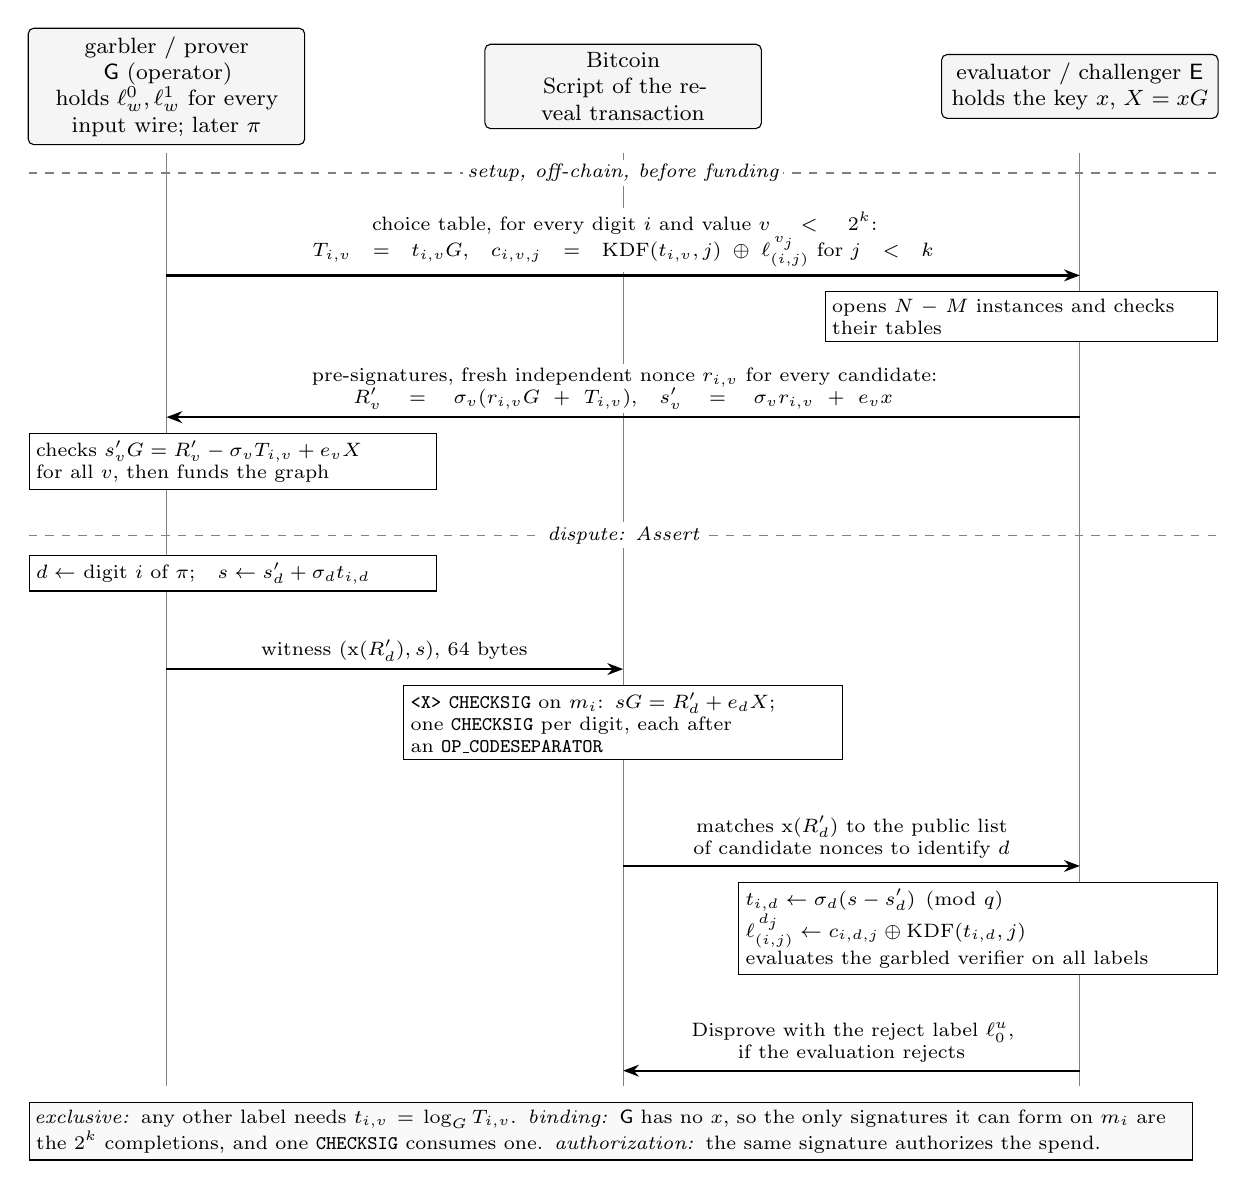
\begin{tikzpicture}[font=\footnotesize, >={Stealth[length=2mm]},
  actor/.style={draw, rounded corners=2pt, fill=gray!8, inner sep=3pt, text width=3.3cm, align=center},
  note/.style={draw, fill=white, inner sep=2.5pt, align=left, font=\scriptsize},
  msg/.style={->, thick},
  lbl/.style={font=\scriptsize, align=center, fill=white, inner sep=1.5pt},
  phase/.style={font=\scriptsize\itshape, fill=white, inner sep=1.5pt}]
\def\xg{0}\def\xc{5.8}\def\xe{11.6}
\node[actor] (G) at (\xg,0) {garbler / prover $\mathsf{G}$ (operator)\\holds $\ell^0_w,\ell^1_w$ for every input wire; later $\pi$};
\node[actor] (C) at (\xc,0) {Bitcoin\\Script of the reveal transaction};
\node[actor] (E) at (\xe,0) {evaluator / challenger $\mathsf{E}$\\holds the key $x$, $X=xG$};
\foreach \x in {\xg,\xc,\xe} \draw[gray] (\x,-0.85) -- (\x,-12.7);
\draw[dashed,gray] (-1.75,-1.1) -- (13.35,-1.1); \node[phase] at (\xc,-1.1) {setup, off-chain, before funding};
\draw[msg] (\xg,-2.4) -- (\xe,-2.4) node[lbl,midway,above=1pt,text width=10.6cm] {choice table, for every digit $i$ and value $v<2^k$:\\ $T_{i,v}=t_{i,v}G$,\quad $c_{i,v,j}=\mathrm{KDF}(t_{i,v},j)\oplus\ell^{\,v_j}_{(i,j)}$ for $j<k$};
\node[note, anchor=north east, text width=4.8cm] at (\xe+1.75,-2.6) {opens $N-M$ instances and checks their tables};
\draw[msg] (\xe,-4.2) -- (\xg,-4.2) node[lbl,midway,above=1pt,text width=10.6cm] {pre-signatures, fresh independent nonce $r_{i,v}$ for every candidate:\\ $R'_v=\sigma_v(r_{i,v}G+T_{i,v})$,\quad $s'_v=\sigma_v r_{i,v}+e_vx$};
\node[note, anchor=north west, text width=5.0cm] at (\xg-1.75,-4.4) {checks $s'_vG=R'_v-\sigma_vT_{i,v}+e_vX$\\for all $v$, then funds the graph};
\draw[dashed,gray] (-1.75,-5.7) -- (13.35,-5.7); \node[phase] at (\xc,-5.7) {dispute: Assert};
\node[note, anchor=north west, text width=5.0cm] at (\xg-1.75,-5.95) {$d\gets$ digit $i$ of $\pi$;\quad $s\gets s'_d+\sigma_dt_{i,d}$};
\draw[msg] (\xg,-7.4) -- (\xc,-7.4) node[lbl,midway,above=1pt,text width=5cm] {witness $(\mathrm{x}(R'_d),s)$, 64 bytes};
\node[note, anchor=north, text width=5.4cm] at (\xc,-7.6) {\texttt{<X> CHECKSIG} on $m_i$: $sG=R'_d+e_dX$;\\one \texttt{CHECKSIG} per digit, each after\\an \texttt{OP\_CODESEPARATOR}};
\draw[msg] (\xc,-9.9) -- (\xe,-9.9) node[lbl,midway,above=1pt,text width=5cm] {matches $\mathrm{x}(R'_d)$ to the public list\\of candidate nonces to identify $d$};
\node[note, anchor=north east, text width=5.9cm] at (\xe+1.75,-10.1) {$t_{i,d}\gets\sigma_d(s-s'_d)\pmod q$\\$\ell^{\,d_j}_{(i,j)}\gets c_{i,d,j}\oplus\mathrm{KDF}(t_{i,d},j)$\\evaluates the garbled verifier on all labels};
\draw[msg] (\xe,-12.5) -- (\xc,-12.5) node[lbl,midway,above=1pt,text width=5cm] {Disprove with the reject label $\ell^u_0$,\\if the evaluation rejects};
\node[note, anchor=north west, fill=gray!5, text width=14.6cm] at (-1.75,-12.9) {\emph{exclusive:} any other label needs $t_{i,v}=\log_G T_{i,v}$. \emph{binding:} $\mathsf{G}$ has no $x$, so the only signatures it can form on $m_i$ are the $2^k$ completions, and one \texttt{CHECKSIG} consumes one. \emph{authorization:} the same signature authorizes the spend.};
\end{tikzpicture}
\caption{Schnorr adaptor label selection for one $k$-bit digit position $i$,
as in BitVM3 and Mosaic~\cite{bitvm3paper,mosaic26}. $m_i$ is the BIP341~\cite{bip341} message
seen by the $i$-th \texttt{CHECKSIG}; wire $(i,j)$ is bit $j$ of the digit.
Here $G$ is the group generator, $q$ its order, $t_{i,v}$ is the secret
adaptor scalar for candidate $v$, and $v_j$ is bit $j$ of $v$.
The notation $\mathrm{x}(P)$ denotes a point's x-coordinate.
$X$ has even $y$ as in BIP340~\cite{bip340},
$\sigma_v\in\{-1,1\}$ makes $R'_v$ have even $y$, and
$e_v=H_{\mathrm{BIP340}}(\mathrm{x}(R'_v)\,\|\,\mathrm{x}(X)\,\|\,m_i)$.
For each fixed $i$ we suppress $i$ on $R'_v,s'_v,\sigma_v,e_v$.
Every pre-signature uses a fresh independent nonce, including across candidate
values, digit positions and sessions; a zero nonce sum or duplicate candidate
$\mathrm{x}(R'_v)$ is resampled. The candidate nonce list is made public at
setup. Everything above the dispute line is off-chain and repeated for every
digit and every candidate value. In the final step, $u$ indexes the kept garbled instance that rejects.}
\label{fig:adaptorseq}
\end{figure}

\subsection{Hash-based label selection}\label{app:hashsel}

Figure~\ref{fig:hashseq} is the hash-based counterpart of
Figure~\ref{fig:adaptorseq}: the signature completion is replaced by a pair of
hash-chain openings, the evaluator contributes nothing at setup, and the
transaction binding must be added as a separate signature.

\begin{figure}[p]\centering
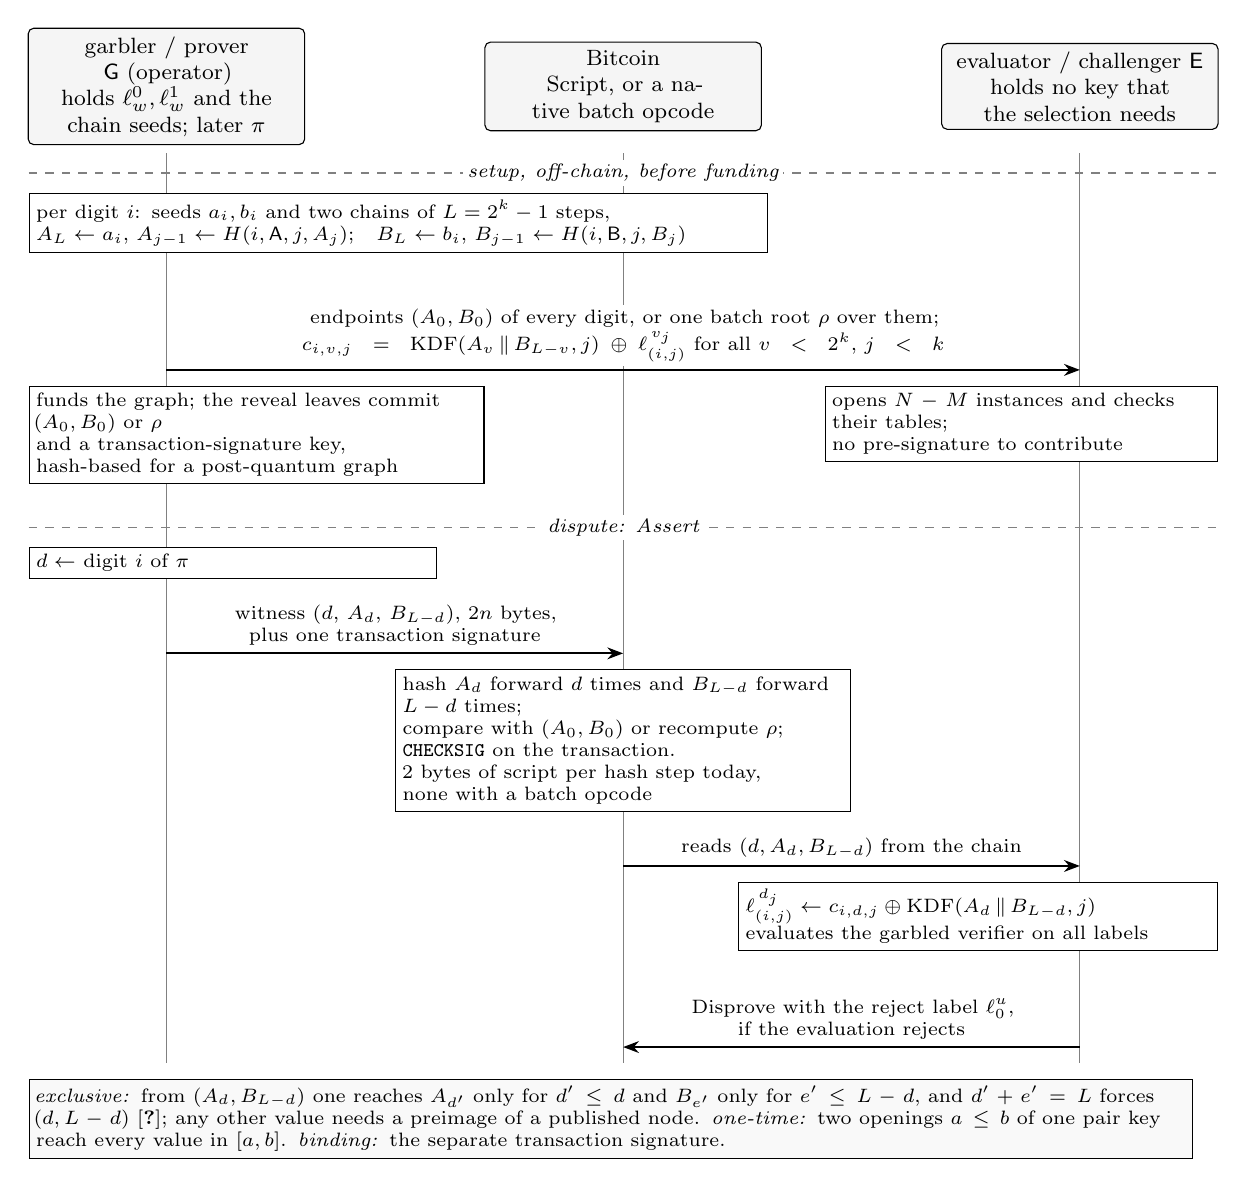
\begin{tikzpicture}[font=\footnotesize, >={Stealth[length=2mm]},
  actor/.style={draw, rounded corners=2pt, fill=gray!8, inner sep=3pt, text width=3.3cm, align=center},
  note/.style={draw, fill=white, inner sep=2.5pt, align=left, font=\scriptsize},
  msg/.style={->, thick},
  lbl/.style={font=\scriptsize, align=center, fill=white, inner sep=1.5pt},
  phase/.style={font=\scriptsize\itshape, fill=white, inner sep=1.5pt}]
\def\xg{0}\def\xc{5.8}\def\xe{11.6}
\node[actor] (G) at (\xg,0) {garbler / prover $\mathsf{G}$ (operator)\\holds $\ell^0_w,\ell^1_w$ and the chain seeds; later $\pi$};
\node[actor] (C) at (\xc,0) {Bitcoin\\Script, or a native batch opcode};
\node[actor] (E) at (\xe,0) {evaluator / challenger $\mathsf{E}$\\holds no key that the selection needs};
\foreach \x in {\xg,\xc,\xe} \draw[gray] (\x,-0.85) -- (\x,-12.4);
\draw[dashed,gray] (-1.75,-1.1) -- (13.35,-1.1); \node[phase] at (\xc,-1.1) {setup, off-chain, before funding};
\node[note, anchor=north west, text width=9.2cm] at (\xg-1.75,-1.35) {per digit $i$: seeds $a_i,b_i$ and two chains of $L=2^k-1$ steps,\\$A_L\gets a_i$, $A_{j-1}\gets H(i,\mathsf{A},j,A_j)$;\quad $B_L\gets b_i$, $B_{j-1}\gets H(i,\mathsf{B},j,B_j)$};
\draw[msg] (\xg,-3.6) -- (\xe,-3.6) node[lbl,midway,above=1pt,text width=10.6cm] {endpoints $(A_0,B_0)$ of every digit, or one batch root $\rho$ over them;\\ $c_{i,v,j}=\mathrm{KDF}(A_v\,\|\,B_{L-v},j)\oplus\ell^{\,v_j}_{(i,j)}$ for all $v<2^k$, $j<k$};
\node[note, anchor=north east, text width=4.8cm] at (\xe+1.75,-3.8) {opens $N-M$ instances and checks their tables;\\no pre-signature to contribute};
\node[note, anchor=north west, text width=5.6cm] at (\xg-1.75,-3.8) {funds the graph; the reveal leaves commit $(A_0,B_0)$ or $\rho$\\and a transaction-signature key,\\hash-based for a post-quantum graph};
\draw[dashed,gray] (-1.75,-5.6) -- (13.35,-5.6); \node[phase] at (\xc,-5.6) {dispute: Assert};
\node[note, anchor=north west, text width=5.0cm] at (\xg-1.75,-5.85) {$d\gets$ digit $i$ of $\pi$};
\draw[msg] (\xg,-7.2) -- (\xc,-7.2) node[lbl,midway,above=1pt,text width=5.2cm] {witness $(d,\,A_d,\,B_{L-d})$, $2n$ bytes,\\plus one transaction signature};
\node[note, anchor=north, text width=5.6cm] at (\xc,-7.4) {hash $A_d$ forward $d$ times and $B_{L-d}$ forward $L-d$ times;\\compare with $(A_0,B_0)$ or recompute $\rho$;\\\texttt{CHECKSIG} on the transaction.\\2 bytes of script per hash step today,\\none with a batch opcode};
\draw[msg] (\xc,-9.9) -- (\xe,-9.9) node[lbl,midway,above=1pt,text width=5cm] {reads $(d,A_d,B_{L-d})$ from the chain};
\node[note, anchor=north east, text width=5.9cm] at (\xe+1.75,-10.1) {$\ell^{\,d_j}_{(i,j)}\gets c_{i,d,j}\oplus\mathrm{KDF}(A_d\,\|\,B_{L-d},j)$\\evaluates the garbled verifier on all labels};
\draw[msg] (\xe,-12.2) -- (\xc,-12.2) node[lbl,midway,above=1pt,text width=5cm] {Disprove with the reject label $\ell^u_0$,\\if the evaluation rejects};
\node[note, anchor=north west, fill=gray!5, text width=14.6cm] at (-1.75,-12.6) {\emph{exclusive:} from $(A_d,B_{L-d})$ one reaches $A_{d'}$ only for $d'\le d$ and $B_{e'}$ only for $e'\le L-d$, and $d'+e'=L$ forces $(d,L-d)$~\cite{antichain26}; any other value needs a preimage of a published node. \emph{one-time:} two openings $a\le b$ of one pair key reach every value in $[a,b]$. \emph{binding:} the separate transaction signature.};
\end{tikzpicture}
\caption{Hash-based label selection for one $k$-bit digit position $i$ with
$n$-byte chain nodes. The selection material is two nodes instead of one
signature, the evaluator contributes nothing at setup, and the transaction
binding that the adaptor gets from the same signature must be added separately.
Verification is a hash ladder, in Script today or in a batch opcode under the
soft fork of Table~\ref{tab:pqsel}. In this figure, $H$ denotes the
domain-separated chain hash, with $\mathsf{A}$ and $\mathsf{B}$ distinguishing
the two chains; the digit index $i$ is suppressed on $A_j,B_j$.
The value $v_j$ is bit $j$ of candidate digit $v$, while $u$ indexes the kept garbled instance that rejects.}
\label{fig:hashseq}
\end{figure}

\subsection{A post-quantum instantiation}\label{app:pqsel}

\paragraph{A post-quantum instantiation.} Figure~\ref{fig:hashseq} becomes
a post-quantum replacement for the adaptor under three changes, none of which
is available on Bitcoin today. First, the forward hashing moves out of Script
into a native batch verifier: one leaf per transaction carries the batch root
$\rho$, the first digit index and the count, and an opcode re-derives every
endpoint from the records on the stack. Second, the transaction-binding
signature becomes hash-based. We model the draft P2MR output
type~\cite{bip360} with a new 0xC2 leaf, 6{,}000-byte stack items and a
548-byte stateful SHRINCS signature~\cite{shrincs} per transaction.
The leaf version and stack limit are assumptions of our serialization model;
548 bytes is the minimum stateful signature size in the SHRINCS draft. Third, the node width $n$ must match the quantum
target: forging a different digit from a published opening is a second-preimage
search over the roughly $2^{22}$ chain nodes that the whole input makes
public, so $n=16$ gives about 53 quantum bits, $n=24$ about 85 and $n=32$ about
117.

We serialized this construction exactly with rust-bitcoin for $n=16$ and
$n=24$ at $k=4$, including the P2MR outputs, 0xC2 leaves, placeholder
signatures, depth-one control blocks and canonical multi-record stack items,
and tested the pair code and the batch parser against tampering, reordering,
cross-batch splicing and padding; nothing in it is executable by Bitcoin Core.
Table~\ref{tab:pqsel} gives the results together with a projection whose model
reproduces both serialized fixtures within $0.03\%$. The operative row is
$n=32$, $k=8$: full-width nodes, about 117 quantum bits for the selection, and
about 2.13\,MvB against the Schnorr adaptor's 2.23\,MvB, at the price of 255 hash steps per
byte inside the opcode, about $3.3\times10^7$ compressions for the input. Its setup is two seeds per digit rather than the adaptor's $2^k$
secrets, so widening $k$ does not grow the choice table; only the translation
table grows, to $2^k\cdot k\cdot 16$ bytes per digit, 4.3\,GB per instance at
$k=8$. The delivery and soldering of that table across the $M$ kept
garblings is the same open item as for every other row.

\begin{table}[t!]\centering\footnotesize\setlength{\tabcolsep}{4pt}
\begin{tabularx}{\textwidth}{>{\raggedright\arraybackslash}p{3.1cm}>{\raggedright\arraybackslash}p{2.5cm}rrrr>{\raggedright\arraybackslash}X}\toprule
selection & consensus & $n$ & $k$ & vB/bit & component & selection security, quantum\\\midrule
Schnorr adaptor (Fig.~\ref{fig:adaptorseq}) & current & -- & 8 & 2.14 & 2.23\,MvB & broken (Shor)\\
WOTS translation~\cite{wotstranslation26} in Script & current & 20 & 3 & 7.59 & 7.90\,MvB & $\approx64$ bits (translation-key chain; nodes $\approx70$)\\
Antichain $(2,16)$ in Script & current & 20 & 4 & 11.41 & 11.88\,MvB & $\approx69$ bits\\
batched selector, one record per item & P2MR, 0xC2, batch opcode & 16 & 4 & 2.05 & 2.13\,MvB & $\approx53$ bits\\
batched selector, 11-record items & same & 16 & 4 & 2.04 & 2.12\,MvB & $\approx53$ bits\\
batched selector, 5-record items & same & 24 & 4 & 3.05 & 3.17\,MvB & $\approx85$ bits\\
batched selector, projected & same & 32 & 8 & $\approx2.05$ & $\approx2.13$\,MvB & $\approx117$ bits\\\bottomrule
\end{tabularx}
\caption{Hash-based label selection against the adaptor baseline for the
1{,}041{,}024-bit input, funding plus reveals. The first three rows are the
independent Core-tested publication fixtures at this payload size. The batched-selector rows are
exact rust-bitcoin serializations of a construction that requires the draft
P2MR output, a hash-based transaction signature and a hypothetical batch
verification opcode; the last row is a model projection. The security column
is the multi-target second-preimage cost of the chain nodes alone (the
20-byte Antichain nodes expose roughly $2^{23}$ chain targets at this
payload size), except for WOTS translation, whose 128-bit key chain gives the lower bound; the
composed protocol remains bound by the proof system (\S\ref{sec:pq}).}
\label{tab:pqsel}
\end{table}

\subsection{The four input schemes}\label{app:schemes}

The four one-time schemes of Table~\ref{tab:ziren-publication} trade
on-chain size against assumptions. The totals in this subsection use the
final WHIR verifier's 564{,}552-bit input.
\begin{itemize}
  \item \emph{Lamport.} Each bit has two hashed 16-byte preimages, and the
    revealed preimage is the one-time-signature witness. The leaf script
    per bit,
    \begin{center}\ttfamily\small OP\_HASH160 OP\_DUP $h_0$ OP\_EQUAL OP\_SWAP $h_1$ OP\_EQUAL OP\_BOOLOR OP\_VERIFY\end{center}
    uses $h_0,h_1$ for the hashes of the two preimages. It is 49 bytes,
    and the witness 17 bytes. We executed it with 998 bits per
    input, and it rejected wrong preimages. The transaction-bound fixture
    prefixes each leaf with a 32-byte authorization key and
    \texttt{OP\_CHECKSIGVERIFY}, and supplies a 64-byte
    \texttt{SIGHASH\_DEFAULT} signature. Its initial stack has 999 items and
    the measured transient peak is exactly the 1{,}000-item Tapscript
    limit~\cite{bip342}. Its serialized size is the Lamport row of
    Table~\ref{tab:ziren-publication}. The fixture uses a one-leaf tree with a 33-byte
    control block; timeout siblings and their longer control paths belong to
    the missing complete graph.
  \item \emph{Antichain Winternitz.} Plain Winternitz chains are unsafe here: from
    a published chain value the evaluator hashes forward to the labels of other
    digit values~\cite{antichain26}. Antichain Winternitz closes this and costs
    a cited marginal $11.31$\,vB per bit at parameters $(2,16)$, counting the
    hash-chain opening witness and authentication script but cancelling fixed
    transaction overhead. Our transaction-bound fixture pins the upstream
    implementation, prepends a 64-byte Schnorr authorization, and includes two
    pay-to-Taproot (P2TR) outputs, input shells, leaf scripts and depth-zero
    controls. With at most 332 four-bit digits per input, its size is the
    Antichain row of Table~\ref{tab:ziren-publication}, an all-nonzero worst case that
    zero-valued ScriptNum coordinates only reduce. The source
    reports $0.256$\,kB of off-chain table per bit. Its
    larger parameters save more on-chain but need up to $43.8$\,kB per bit
    off-chain~\cite{antichain26}.
  \item \emph{Winternitz with a translation table.} The translation gadget
    of~\cite{wotstranslation26} also closes the gap of plain Winternitz: each label is a Shamir
    secret whose threshold is set by the chunk's checksum and the bit value, so
    a signed chunk opens exactly the labels of its bits. In the source, one
    such Winternitz signature over 508 bits, its Assert, is 3{,}748\,vB, or
    $7.38$\,vB per bit. Our transaction-bound fixture
    uses 3-bit digits, eight per chunk, with the checksum split over two
    chains, and the authorization, outputs and controls of the Antichain
    fixture. With at most 49 chunks per input, its size is the WOTS row of
    Table~\ref{tab:ziren-publication}, again an all-nonzero worst case. The price is the
    off-chain table, 1{,}033{,}130{,}160 bytes per instance at this input size. The challenger must decode digits as consensus
    does and, at setup, reject keys in which one chain end lies within seven
    hashes of another; neither check costs on-chain space.
  \item \emph{Schnorr adaptor signatures} over 8-bit digits, as in BitVM3 and
    Mosaic. BitVM3 reports 9{,}707 weight units (WU) for a 1{,}024-bit Assert
    transaction with one input and two P2TR outputs~\cite{bitvm3paper}, or
    $2.37$\,vB per bit at that size. Its printed witness formula instead sums to
    9{,}451 WU once the SegWit marker and flag are included, while the merged
    64-byte-\texttt{SIGHASH\_DEFAULT} implementation implies 9{,}323 WU for
    that shell. Our executable fixture reproduces 9{,}323 WU, uses the BIP342
    opcode index rather than a byte offset for every code separator, and reaches
    the exact 998-signature stack capacity. Core 31.1 validates all completed
    signatures. The final-input serialization uses 70{,}569 eight-bit digits;
    its size is the adaptor row
    of Table~\ref{tab:ziren-publication}. Mosaic's source construction solders all
    kept instances to one set of signatures by polynomial label correlation,
    with an on-chain footprint independent of the number of
    instances~\cite{mosaic26}. This repository tests only the one-key-set
    transaction fixture; it does not implement or test Mosaic's polynomial
    correlation or setup verification. The signatures rest on
    discrete logarithms, and an evaluator that holds the signing key can spend
    without completing the adaptor~\cite{antichain26}.
\end{itemize}
% =====================================================================
\section{Additional measurements}\label{app:eval}

\subsection{Artifact availability}\label{app:artifact}

\paragraph{Artifact availability.} The source repository includes the locked
dependencies and benchmark commands; the commands and memory caps are listed in
\texttt{whir-gc/README.md}. The measurement logs and helper sources are included in
\texttt{paper/data/}, together with a SHA-256 manifest and a README mapping
tables and figures to logs. The level-2 row of Table~\ref{tab:recursion} was measured at Ziren
\texttt{f6137ecc} with 26-bit address and permutation identifiers. The later
optimized measurements are associated with Ziren \texttt{9398469a} on the
unpublished \texttt{whir-gc/narrow-verifier-input} branch, with subsequent
experimental patches. Although the branch reference
is no longer available, its base commit survives in the local Git object
database, including the dumper test and 64-byte rewiring rows. Cumulative
patches preserved at this repository's revision \texttt{8359bb0} apply
cleanly to that base and to Plonky3 \texttt{fb5d0d89}. The script
\texttt{patches/reconstruct\_historical.py} reconstructs those trees and emits
a file-checksum manifest. The archival notes associate these patches with
the measurements; no original final-tree hash is available to confirm that
association independently. The public reconstruction uses Ziren
\texttt{80af2779} on \texttt{feat/binary-whir-blake3} and Plonky3
\texttt{be1c6f92} on ProjectZKM's \texttt{zkm/binary-whir}. It has a rewritten
dumper and lacks the original rewiring-row implementation, so rebuilding
from these public commits does not reproduce the reported level-4 counts
exactly. The available archive contains the final gate-count, value-check,
mutation and streaming-garbling log, but no checksummed level-4 proof/tape
pair from that run. Consequently, these logs support auditing the reported
observations, not independently replaying the exact circuit. Reproduction
requires either recovery of that pair and its recorder/configuration manifest,
or a new measurement on the public reconstruction with separately reported
counts. \texttt{patches/README.md} documents the reconstruction and commands.
Gate, wire and input counts are deterministic.

\subsection{Narrow recursion}\label{app:recursion}

Table~\ref{tab:recursion} in \S\ref{sec:eval} lists every verifier of the
narrow-recursion cost analysis; from the third row on, each is a level-4 proof
re-proved from the same level-3 tape at the Johnson rate $1/1024$ and
re-recorded. The tape machine can bind up to eight of a tape's first inputs as
public values, enough for the binary stage's public-value digest, which commits
to the zkVM program's verifying key and outputs; our runs bind none. We
translate a tape gate by gate in the \texttt{binary\_tape} module of
\texttt{whir-gc}, and Ziren's \texttt{binary-recursion} crate records the
tapes.


Section~\ref{sec:reduce} describes the layout, recording, opening and
commitment optimizations used in these configurations. Here we give their
algebraic conditions and the remaining security obligations. The archived
tests exercise honest and tampered inputs; they do not prove soundness.
Appendix~\ref{app:artifact} documents the public reconstruction and its
differences from the measurement version.

\paragraph{Algebraic reductions and their scope.}
Write $q=|\F|$. The following arguments concern the interactive algebraic
reductions, conditional on fixed statement shapes, correctly derived linear
forms and fresh uniform challenges after the preceding messages are fixed.
They do not establish round-by-round soundness of the complete composition
or its Fiat--Shamir transform. When a commitment admits several candidate
traces, the error must also account for that candidate set.

\paragraph{Merged tensors and the joint switch.}
When the absorbed coordinates agree, all claims use the same linear map
$\ell$ from a ring-switch tensor to its claimed value. For $m$ tensors $T_i$
and claimed readings $y_i$, with $0\le i<m$, sample $\mu$ uniformly from
$\F$ after fixing the readings. The merged tensor is
$T=\sum_{i=0}^{m-1}\mu^i T_i$, and the verifier checks
$\ell(T)=\sum_i\mu^i y_i$. For any fixed nonzero discrepancy vector,
$\sum_i\mu^i(\ell(T_i)-y_i)$ has degree at most $m-1$, giving error at most
$(m-1)/q$. The subsequent tensor checks and sumcheck must still bind $T$ to
the packing; their errors are additional. The implementation checks equality
of the absorbed coordinates and disallows successor views in the merged
case. Its outer opening transcript binds the claimed forms and column folds
before the ring switch draws $\mu$; the ring-switch transcript then binds
$T$ before drawing its tensor-batching point. The standalone ring-switch
routine relies on that prior binding of readings.

The joint switch concatenates two equal-size packed tables. If their
multilinear extensions are $P_0$ and $P_1$, its polynomial is
$P(s,z)=(1-s)P_0(z)+sP_1(z)$. Original claims are embedded at $s=0$ or $s=1$.
At the terminal point $(s^*,z^*)$, the verifier authenticates both
$P_0(z^*)$ and $P_1(z^*)$ through the paired WHIR opening and checks their
selector-weighted sum against the ring-switch value. This is an exact
identity; security still includes the ring-switch error at the enlarged
arity and the paired opening's error.

\begin{lemma}[Linear-form reconstruction]\label{lem:forms}
Let $L$ be a fixed matrix and $R$ a right inverse on its image. Suppose each
constraint and bus expression affected by the substitution factors as
$P(x,u)=\widehat P(Lx,u)$, with $u$ denoting the unchanged operands. Then
replacing $x$ by $R(Lx)$ preserves all those expressions. Affine identities
among forms of a fixed preprocessed trace also hold at every multilinear
evaluation point if they hold at every row of that trace.
\end{lemma}
\begin{proof}
The first claim follows from $LR(Lx)=Lx$. For the second, multilinear
extension is linear, and the extension of the all-ones column is the
constant polynomial 1. Thus, for vectors $f,g$ of preprocessed forms, a
fixed coefficient matrix $A$ and a constant vector $c$, an identity
$f=Ag+c$ on the Boolean row domain extends to $f(r)=Ag(r)+c$ at every
row evaluation point $r$.
\end{proof}
The implementation derives the forms from symbolic constraints and bus
expressions, and checks the right-inverse identities. For preprocessed
forms, the affine relations are derived from the fixed trace. This lemma
explains the substitution; validating the symbolic extractor and binding
the transmitted forms to committed columns remain implementation obligations.

\begin{lemma}[Shared forms sumcheck]\label{lem:shared-forms}
Suppose $m_{\mathrm{form}}$ claimed forms, their row points and the relevant
commitments are fixed before a uniform challenge $\rho\in\F$. Let
$d_{\mathrm{col}}$ be the largest column-variable count, and assume the
commitments admit at most $K$ candidate collections
of column evaluations before $\rho$. A degree-two sumcheck over the
zero-extended column tables reduces these claims to authenticated column
folds with algebraic error at most
$K(m_{\mathrm{form}}-1+2d_{\mathrm{col}})/q$, in addition to the error of
authenticating those folds.
\end{lemma}
\begin{proof}
For a fixed candidate collection, let $\delta_j$ be claimed form $j$ minus
its candidate evaluation. A false vector of forms gives a nonzero
polynomial $\sum_{j=0}^{m_{\mathrm{form}}-1}\rho^j\delta_j$, which vanishes with probability
at most $(m_{\mathrm{form}}-1)/q$. Otherwise the initial weighted claim is false. Each
round checks a polynomial of degree at most two, so the usual sumcheck
induction adds at most $2d_{\mathrm{col}}/q$ before a false terminal claim remains.
Union-bounding over the $K$ candidate collections gives the stated term.
\end{proof}
For a table $t$ with $k_t$ column variables and a terminal point
$z\in\F^{d_{\mathrm{col}}}$, let
$b_t(z)=\prod_{i=1}^{d_{\mathrm{col}}-k_t}(1-z_i)$ and let $z_t$ be the trailing $k_t$
coordinates of $z$. Zero extension multiplies both its column polynomial $C_t$
at the fixed row point and its batched form-weight polynomial $W_t$ by
$b_t$. Writing $S$ for the combined sumcheck integrand, the terminal check
must be
\[
  S(z)=\sum_t b_t(z)^2 W_t(z_t)C_t(z_t).
\]
The implementation uses this squared prefix factor, binds every table's
forms before drawing $\rho$, and absorbs each round's two coefficients
before sampling its coordinate. Each $C_t(z_t)$ then becomes a ring-switch
claim. A concrete assessment must charge the total number $m_{\mathrm{form}}$ of forms and
the applicable candidate multiplicity; the previous column-batching term
cannot be reused solely because the transcript is shorter.

\paragraph{Eq-factored bus rounds.}
A radix-four product layer still uses one-variable Boolean sumcheck rounds.
Its degree-five round polynomial is $g(X)=e_r(X)h(X)$, where
$e_r(X)=(1-r)(1-X)+rX$ and $\deg h\le4$; $r$ is the current coordinate of
the equality-polynomial challenge point. Given running claim
$s=g(0)+g(1)$ and next sumcheck challenge $\alpha\in\F$, the verifier
reconstructs the omitted value as
\[
  h(1)=\frac{s-(1-r)h(0)}{r},\qquad
  s'=e_r(\alpha)h(\alpha).
\]
Here $s'$ is the updated claim. For $r\ne0$, this enforces $g(0)+g(1)=s$
exactly. The round message is
absorbed before $\alpha$ is sampled, so the degree-five sumcheck argument
still applies; omitting a transmitted value does not itself reduce that
error bound. The implementation rejects $r=0$, introducing a completeness
loss of at most $n_{\mathrm{guard}}/q$ for $n_{\mathrm{guard}}$ such coordinates under uniform challenges.
This guard contributes to the recursion path's completeness loss.

\paragraph{Collision accounting and composition.}
Both the reconstructed historical source and the public reconstruction use
25-byte Merkle digests but return 128 from
\texttt{collision\_resistance\_bits}. That metadata is inconsistent with
the digest width: generic collision work is about $2^{100}$ classically
and $2^{200/3}$ quantumly. The accompanying correction derives the metadata
from the digest width in both native and traced configurations. This affects
the security report, not the historical gate counts. Accordingly, the
previously reported 100-bit per-proof calculator estimates must be
recomputed with the corrected cap and the new reduction terms; they are not
certified bounds for the modified protocol. The full analysis must also
instantiate the candidate-set charges, tensor and paired-opening reductions,
round-by-round soundness, hash errors and the recursive composition. Because the circuit checks only the last proof, the
statement's soundness also composes over the earlier levels and over the zkVM
proof itself. For the zkVM proof, Ziren reports more than 100 bits of
interactive soundness per proof stage and 93.5 bits for an illustrative tree of
150 proofs in the Poseidon2 configuration evaluated in that
paper~\cite{duan26ziren}. These figures concern that configuration's
interactive soundness.

At 564{,}552 bits, the input-publication fixtures of Table~\ref{tab:ziren-publication},
with every transaction signed and every leaf executed under the stack limit,
have total virtual sizes of 1{,}205{,}217\,vB for the 8-bit adaptor baseline (73 inputs in 13
reveal transactions), 4{,}263{,}180\,vB for WOTS translation (481 inputs in 44),
6{,}425{,}757\,vB for Antichain $(2,16)$ (426 inputs in 71) and
9{,}363{,}254\,vB for Lamport (566 inputs in 95, plus a 7{,}155\,vB join);
Disprove is one 97\,vB transaction. Plain 4-bit Winternitz, modeled from one
executed input at 23.06 weight units per bit, would be about 3.26\,MvB, but it
cannot deliver garbled labels without a translation table, which for WOTS
translation costs 1.03\,GB per instance at this input. The accounting boundary
is that of Table~\ref{tab:ziren-publication}.

% =====================================================================
\section{Security details}\label{app:security}

This appendix derives the component-level estimates in Table~\ref{tab:pq}
and explains the QROM accounting used in \S\ref{sec:security}. The recursive
proof's algebraic and composition obligations appear in Appendix~\ref{app:recursion}.

\paragraph{Hash-based input keys under multi-target search.} The protocol
of \S\ref{sec:dispute} publishes input bits under one-time keys. Lamport, Antichain Winternitz and
translated Winternitz keys rest on \texttt{HASH160} preimages. The familiar $2^{64}$ quantum cost for our
16-byte preimages is a single-target estimate. One Lamport key set exposes
$T=564{,}552$ alternative preimages for the final verifier input, so generic
multi-target search costs about $2^{128}/T\approx2^{108.9}$ classically and
$\sqrt{2^{128}/T}\approx2^{54.4}$ quantumly. Seven independent sets lower
these figures to about $2^{106.1}$ and $2^{53.0}$. Hash-chain alternatives have the
same multi-target issue; Table~\ref{tab:pqsel} gives the widths that lift the
selection itself above this bound. Even 20-byte preimages under \texttt{HASH160} are
capped near 70 quantum bits for one set, rather than 80, once the target count
is included. Translated Winternitz keys are further bounded by the 128-bit key
chain of the translation table. Because each step of that chain is salted with
the instance, the chunk and the step index, an inversion targets a single step,
and its cost is $2^{128}$ classically and $2^{64}$ quantumly.

\paragraph{Fiat--Shamir against quantum adversaries.} Chiesa, Manohar and
Spooner~\cite{cms19qrom} give a QROM Fiat--Shamir reduction for suitable
public-coin interactive oracle proofs with round-by-round soundness. In the
form used here its error is
$O(t^2\varepsilon_{\mathrm{rbr}}+t^3/2^{\lambda})$, where $\lambda$ is
the hash-output length for the random oracle modeled in the reduction. The corresponding classical accounting includes both a term
linear in $t\varepsilon_{\mathrm{rbr}}$ and hash-related errors; constants and
protocol-dependent factors must be retained for a concrete bound.
WHIR proves round-by-round soundness~\cite[\S5]{whir25}. Extending this
accounting to the implemented composition requires checking every algebraic
layer and the transcript, not just invoking WHIR's theorem.

If a valid round-by-round bound is $2^{-a}$, the expression above remains
small for $t$ sufficiently below both $2^{a/2}$ and $2^{\lambda/3}$, up to its
constants. It supplies no converse: once the bound becomes uninformative,
the existence of a successful attack does not follow. In particular, a
Schwartz--Zippel bound is an upper bound on bad-challenge density. Grover
search gives a matching attack only when a searchable set of successful
challenges of the asserted density is actually available to the adversary.

\paragraph{The garbling.} Authenticity rests on the secrecy of $\Delta$, and
$\Delta$ can be tested against a single gate. An evaluator holding the labels
$a,b$ of an \AND{} gate with known values $x,y$ and its ciphertext $\mathit{ct}$
checks a candidate $\Delta'$ by recomputing $\mathit{ct}$ from
$a,a\oplus\Delta',b$ and $\Delta'$. A wrong candidate passes with probability
$2^{-128}$. Grover search therefore recovers $\Delta$ with about $2^{64}$
quantum evaluations of Blake3, after which every label's complement is known
and the output label of the other value is free. With 128-bit labels the
garbling offers about 64 bits against a quantum adversary. The same holds for a
hashlock on a 128-bit output label: a preimage search over $2^{128}$ labels costs
about $2^{64}$. Grover search is highly sequential, and the adversary has only the
time between setup and the end of the dispute window, but we do not rely on
this.

\end{document}
